% !TeX root = main.tex
%% 
%% Copyright 2007-2020 Elsevier Ltd
%% 
%% This file is part of the 'Elsarticle Bundle'.
%% ---------------------------------------------
%% 
%% It may be distributed under the conditions of the LaTeX Project Public
%% License, either version 1.2 of this license or (at your option) any
%% later version.  The latest version of this license is in
%%    http://www.latex-project.org/lppl.txt
%% and version 1.2 or later is part of all distributions of LaTeX
%% version 1999/12/01 or later.
%% 
%% The list of all files belonging to the 'Elsarticle Bundle' is
%% given in the file `manifest.txt'.
%% 

%% Template article for Elsevier's document class `elsarticle'
%% with numbered style bibliographic references
%% SP 2008/03/01
%%
%% 
%%
%% $Id: elsarticle-template-num.tex 190 2020-11-23 11:12:32Z rishi $
%%
%%
% \documentclass[preprint,12pt]{elsarticle}

%% Use the option review to obtain double line spacing
%% \documentclass[authoryear,preprint,review,12pt]{elsarticle}

%% Use the options 1p,twocolumn; 3p; 3p,twocolumn; 5p; or 5p,twocolumn
%% for a journal layout:
%% \documentclass[final,1p,times]{elsarticle}
%% \documentclass[final,1p,times,twocolumn]{elsarticle}
%% \documentclass[final,3p,times]{elsarticle}
% \documentclass[final,3p,times,twocolumn]{elsarticle}
%% \documentclass[final,5p,times]{elsarticle}
\documentclass[final,5p,times,twocolumn, fleqn]{elsarticle}

%% For including figures, graphicx.sty has been loaded in
%% elsarticle.cls. If you prefer to use the old commands
%% please give \usepackage{epsfig}

%% The amssymb package provides various useful mathematical symbols
\usepackage{amssymb}
\usepackage{amsmath}
\usepackage{algorithmic}
\usepackage{algorithm}
\usepackage{enumerate}
\usepackage{array}
\usepackage{booktabs}
\usepackage{multirow}
\usepackage{tabularx}
\usepackage{xcolor}
\usepackage{hyperref}
\usepackage{lineno}
\usepackage{float}
\usepackage{caption}
\usepackage{cuted}
\setlength{\linenumbersep}{3pt}
\hyphenpenalty=1000
\hypersetup{
     colorlinks   = true,
     linkcolor    = blue,
     citecolor    = blue
}
\setlength{\mathindent}{0pt}
% \newenvironment{revblock}
%   {\begingroup\ifdefined\makeunmarked\else\color{red}\fi}
%   {\endgroup}

% \ifdefined\makeunmarked
%   \RenewDocumentCommand{\textcolor}{O{} m m}{#3}
% \fi

\captionsetup[table]{
  labelfont=bf,             % "Table n" 加粗
  singlelinecheck=false,    % 强制左对齐（禁止单行居中）
  justification=raggedright, % 文本左对齐
  labelsep=newline          % 如果希望 Table 1 和标题文字分两行显示，请取消此行注释
}

\makeatletter
\setlength{\@fptop}{0pt}
\setlength{\@dblfptop}{0pt}
\makeatother
%% The amsthm package provides extended theorem environments
%% \usepackage{amsthm}

%% The lineno packages adds line numbers. Start line numbering with
%% \begin{linenumbers}, end it with \end{linenumbers}. Or switch it on
%% for the whole article with \linenumbers.
%% \usepackage{lineno}

\journal{Journal of Building Engineering}

\begin{document}
\setlength{\abovedisplayskip}{5pt}
\setlength{\belowdisplayskip}{5pt}

\begin{frontmatter}

%% Title, authors and addresses

%% use the tnoteref command within \title for footnotes;
%% use the tnotetext command for theassociated footnote;
%% use the fnref command within \author or \address for footnotes;
%% use the fntext command for theassociated footnote;
%% use the corref command within \author for corresponding author footnotes;
%% use the cortext command for theassociated footnote;
%% use the ead command for the email address,
%% and the form \ead[url] for the home page:
%% \title{Title\tnoteref{label1}}
%% \tnotetext[label1]{}
%% \author{Name\corref{cor1}\fnref{label2}}
%% \ead{email address}
%% \ead[url]{home page}
%% \fntext[label2]{}
%% \cortext[cor1]{}
%% \affiliation{organization={},
%%             addressline={},
%%             city={},
%%             postcode={},
%%             state={},
%%             country={}}
%% \fntext[label3]{}

\title{Calibrated Surrogate-Assisted Optimization for FEA-Efficient Shear Wall Structural Design}

%% use optional labels to link authors explicitly to addresses:
%% \author[label1,label2]{}
%% \affiliation[label1]{organization={},
%%             addressline={},
%%             city={},
%%             postcode={},
%%             state={},
%%             country={}}
%%
%% \affiliation[label2]{organization={},
%%             addressline={},
%%             city={},
%%             postcode={},
%%             state={},
%%             country={}}

\author{Hao Leng\fnref{firstauthor}}
\author{Yuqing Gao\fnref{firstauthor}}
\fntext[firstauthor]{These authors contributed equally to this work and are considered co-first authors}
\author{Ying Zhou\corref{cor}}

\ead{yingzhou@tongji.edu.cn}
\cortext[cor]{Corresponding author}
\address{State Key Laboratory of Disaster Reduction in Civil Engineering, Tongji University, Shanghai 200092, China}

% \affiliation{organization={State Key Laboratory of Disaster Reduction in Civil Engineering, Tongji University},
%             city={Shanghai 200092},
%             country={China}}

% \affiliation[inst2]{organization={Department Two},%Department and Organization
%             addressline={Address Two}, 
%             city={City Two},
%             postcode={22222}, 
%             state={State Two},
%             country={Country Two}}

\begin{abstract}
Shear wall structural optimization for high-rise buildings requires repeated finite-element analysis and code-based design checking, making conventional optimization computationally expensive in preliminary design. Existing surrogate-assisted optimization methods can reduce evaluation cost, but static global surrogates may suffer from layout-specific prediction bias and become unreliable under direct application. This paper proposes a calibrated surrogate-assisted optimization framework for FEA-efficient shear wall structural design. A layout-conditioned surrogate model is first developed to estimate candidate feasibility and reinforcement usage from room-level graph representations, global layout statistics, and design parameters. During optimization, the surrogate predictions are further corrected through online local calibration using FEA-verified samples accumulated from the current layout, enabling layout-specific feasibility probability calibration and reinforcement residual correction. Based on the calibrated predictions, the framework conservatively filters low-feasibility candidates and prioritizes promising low-cost candidates for true FEA evaluation, thereby reallocating the limited analysis budget. Experiments on 143 engineering shear wall layouts with approximately 715,000 FEA-labeled samples show that the proposed method improves candidate assessment, reduces local surrogate bias, and substantially decreases true FEA calls while maintaining comparable solution quality. The results demonstrate that online local calibration and surrogate-assisted budget allocation provide an effective strategy for improving the computational efficiency of shear wall structural optimization.
\end{abstract}

%%Graphical abstract
% \begin{graphicalabstract}
% \includegraphics{grabs}
% \end{graphicalabstract}

%%Research highlights
% \begin{strip}
\begin{highlights}
\item Calibrated surrogates accelerate shear wall structural optimization.
\item Layout-conditioned surrogates predict feasibility and reinforcement demand.
\item Online calibration adapts predictions to each layout and search region.
\item Candidate screening and ranking improve FEA budget allocation.
\end{highlights}
% \end{strip}

\begin{keyword}
%% keywords here, in the form: keyword \sep keyword
Shear wall structures \sep Structural optimization \sep Surrogate-assisted optimization \sep Online local calibration \sep FEA budget allocation

%% PACS codes here, in the form: \PACS code \sep code
% \PACS 0000 \sep 1111
%% MSC codes here, in the form: \MSC code \sep code
%% or \MSC[2008] code \sep code (2000 is the default)
% \MSC 0000 \sep 1111
\end{keyword}

\end{frontmatter}

\linenumbers

%%%%%%%%%%%%%%%%%%%%%%% main body start %%%%%%%%%%%%%%%%%%%%%%
\section{Introduction}
\label{sec:intro}

Surrogate-assisted optimization has become an important strategy for accelerating structural design problems that require repeated finite-element analysis (FEA). In shear wall structural design for high-rise buildings, engineers need to determine wall thicknesses, beam section dimensions, material grades, and other design parameters while satisfying multiple code-based constraints, including inter-story drift, torsional response, axial compression ratio, shear-compression ratio, and member reinforcement requirements. For each candidate design, reliable evaluation usually requires parametric modeling, FEA, structural response extraction, and member-level code checking. When population-based optimizers such as genetic algorithms or particle swarm optimization are adopted, a large number of candidate designs must be evaluated, making repeated FEA and code checking the dominant computational bottleneck.

Existing studies have explored various approaches to improve the automation and efficiency of shear wall structural design. Traditional optimization methods, such as genetic algorithms, tabu search, and other metaheuristic algorithms, have been used to search for cost-effective shear wall layouts or section configurations under engineering constraints . More recent studies have introduced prior design knowledge, CAD/BIM-based automatic modeling, machine learning, and generative models into preliminary shear wall design, enabling more efficient layout generation, structural scheme exploration, and data-driven design support . These studies have advanced the automation of shear wall structural design, but many of them still rely on expensive structural analyses to evaluate candidate solutions. Therefore, for section and material optimization of a given shear wall layout, the key challenge is not only how to search the design space, but also how to allocate limited FEA evaluations to candidates that are more likely to be feasible and cost-effective.

Surrogate models provide a natural way to reduce the number of expensive evaluations in structural optimization. Response surface models, Kriging models, support vector machines, neural networks, and other data-driven surrogates have been widely used to approximate structural responses, replace costly simulations, or guide optimization and reliability analysis . In building engineering, surrogate models have also been applied to predict seismic responses, wind-induced responses, material quantities, and performance indicators of structural systems. These methods demonstrate the potential of data-driven prediction for accelerating structural design. In shear wall structural optimization, a single static surrogate has difficulty reproducing the coupled global and member-level checks that govern design feasibility.

Several limitations become particularly important when surrogate models are used for shear wall structural optimization. First, the behavior of shear wall buildings is strongly layout-dependent. Even under the same section and material parameters, different wall arrangements may lead to different lateral stiffness distributions, load paths, seismic responses, and reinforcement demands. A global surrogate trained on multiple layouts may therefore suffer from layout-specific prediction bias when applied to a new design case. Second, optimization is an iterative process in which the candidate distribution gradually changes. A surrogate model trained offline may not remain accurate in the local region explored by the optimizer. Third, different surrogate predictions should serve different roles in the optimization process. Feasibility prediction should be conservative to avoid rejecting potentially feasible designs, whereas reinforcement usage prediction is more useful for ranking candidates by material economy. These requirements are not fully addressed by conventional surrogate modeling settings that focus mainly on global classification or regression accuracy.

This paper proposes a calibrated surrogate-assisted optimization framework for FEA-efficient shear wall structural design. The proposed framework uses surrogate models as pre-evaluation tools for candidate screening and analysis budget allocation. A layout-conditioned surrogate model is first trained to estimate candidate feasibility and reinforcement usage from layout information and design parameters. During optimization, FEA-verified samples accumulated from the current layout are further used to perform online local calibration, so that global surrogate predictions can be corrected for the current design case and local search region. The calibrated feasibility and reinforcement predictions are then used to conservatively filter low-value candidates and prioritize promising candidates for true FEA and code checking.

The main contributions of this study are summarized as follows. First, a layout-conditioned surrogate modeling strategy is developed for candidate assessment in shear wall section and material optimization, enabling both feasibility screening and reinforcement usage estimation before FEA. Second, an online local calibration mechanism is introduced to correct layout-specific surrogate bias using FEA-verified samples generated during the optimization process. Third, a calibrated surrogate-assisted optimization framework is established to allocate FEA budgets more effectively through conservative candidate screening and priority ranking.

The remainder of this paper is organized as follows. Section 2 defines the shear wall structural optimization problem and introduces the calibrated surrogate modeling strategy. Section 3 presents the surrogate-assisted optimization framework and the online update mechanism. Section 4 describes the dataset, experimental settings, and evaluation metrics. Section 5 reports and discusses the experimental results. Section 6 concludes the paper and outlines future research directions. % introduction

\begin{figure*}[t]
\centering
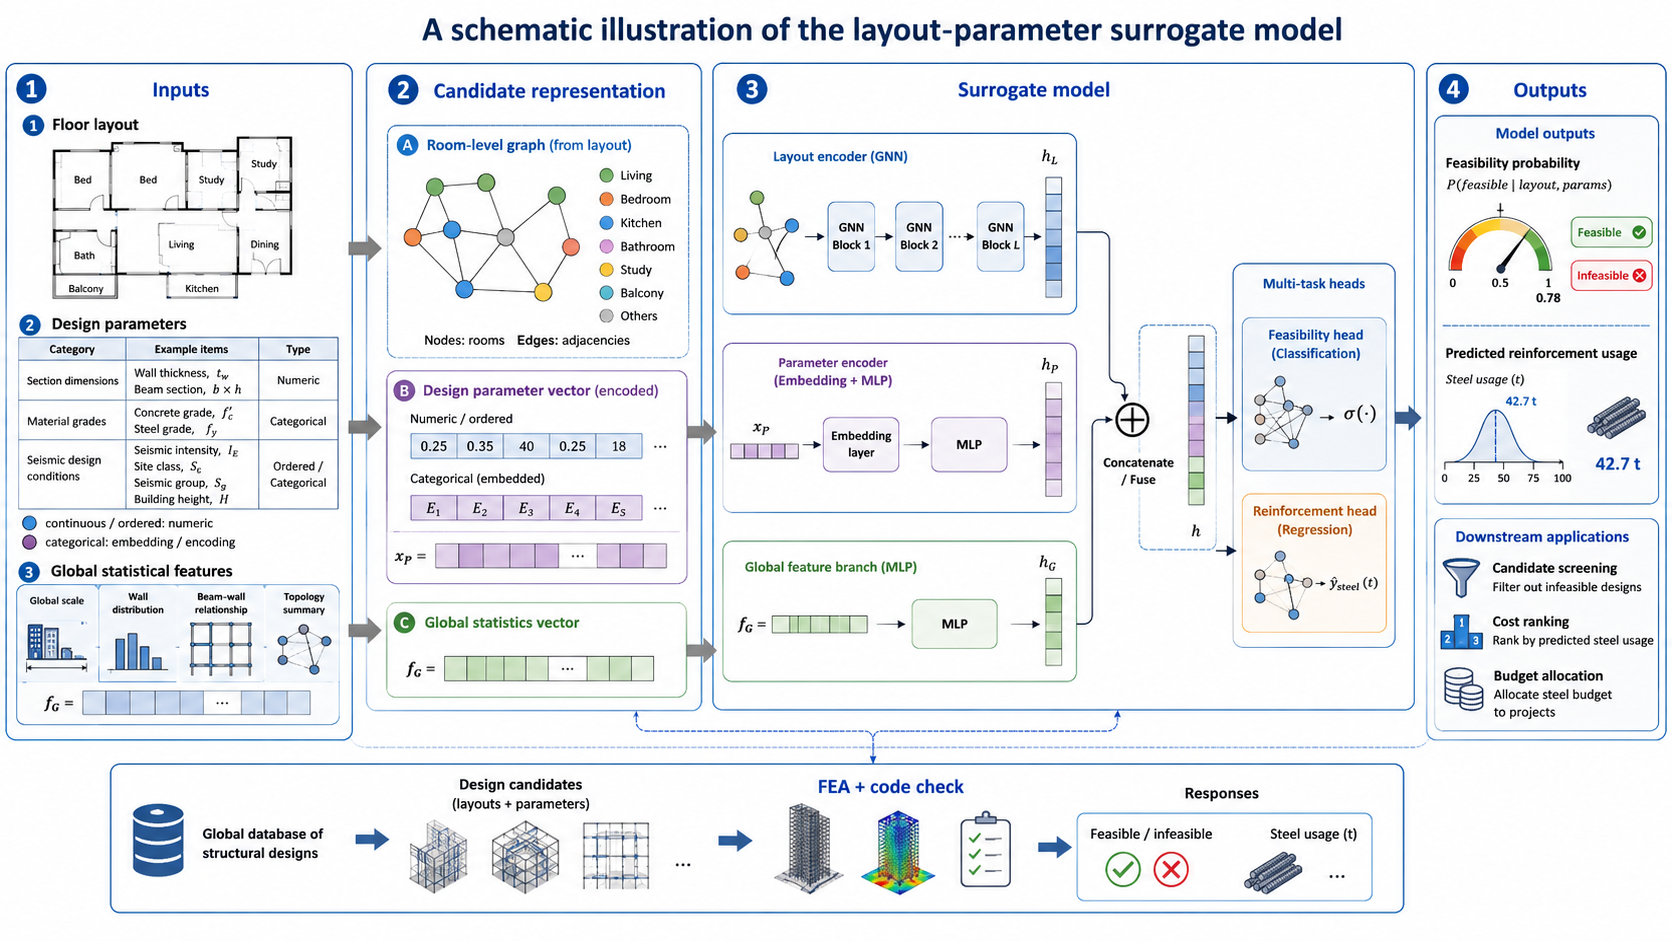
\includegraphics[width=\textwidth]{layout_parameter_surrogate.pdf}
\caption{Layout-conditioned graph surrogate model for candidate feasibility and reinforcement usage prediction.}
\label{fig:layout_parameter_surrogate}
\end{figure*}


\begin{figure*}[t]
\centering
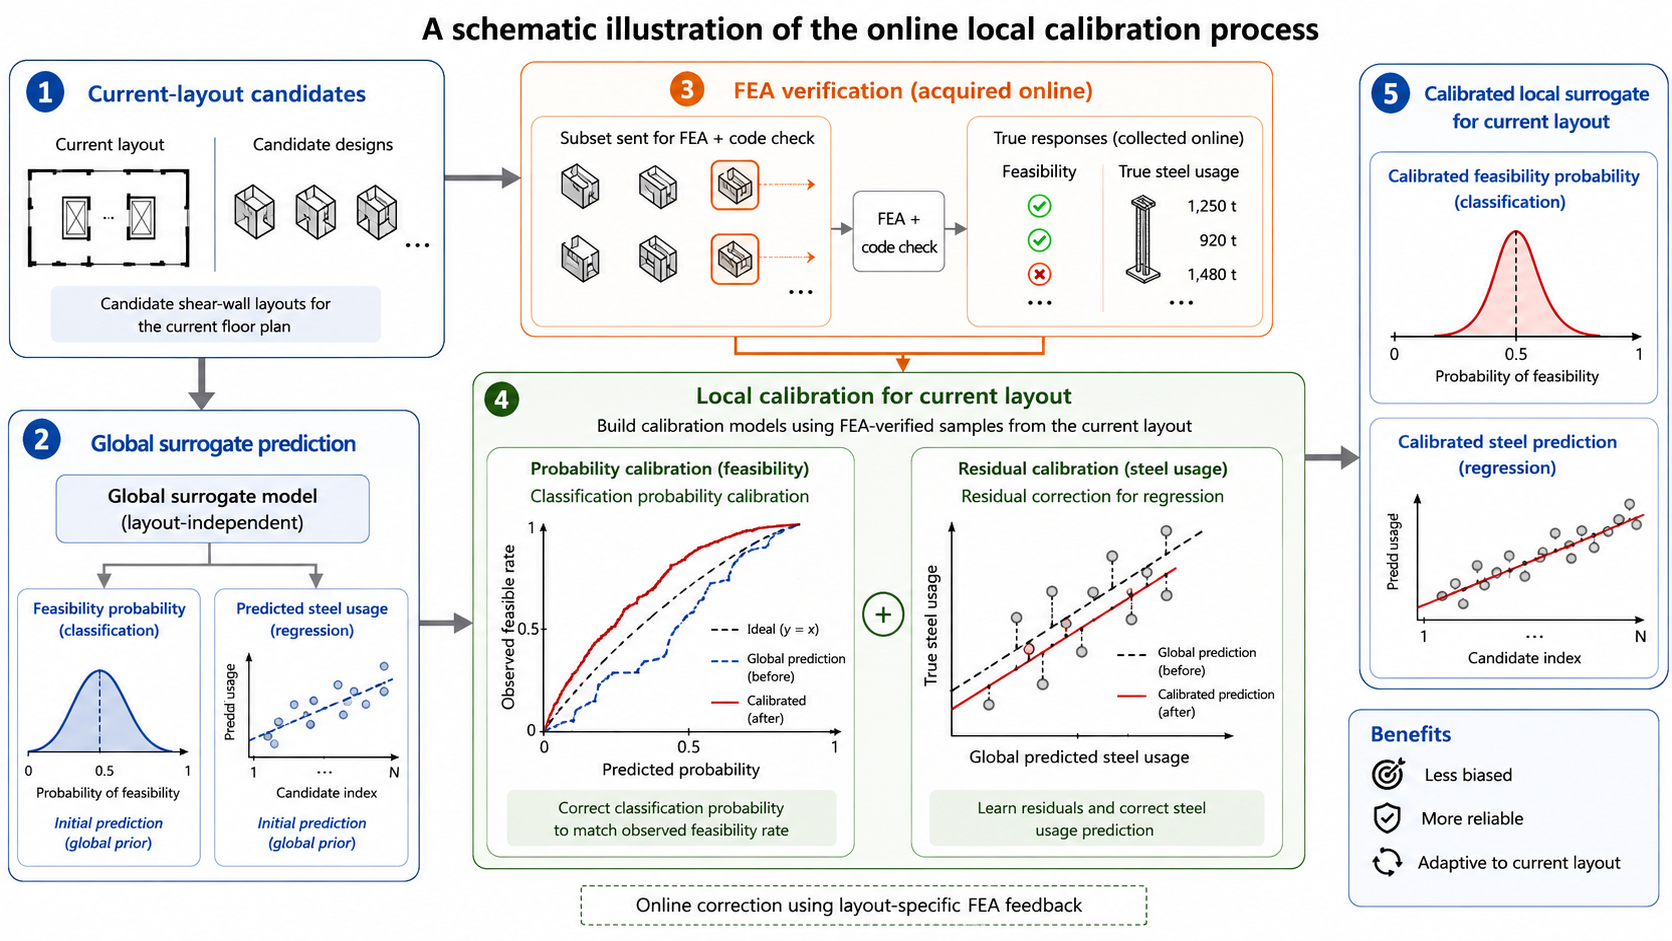
\includegraphics[width=\textwidth]{online_local_calibration.pdf}
\caption{Online local calibration of global surrogate predictions using FEA-verified samples from the current layout.}
\label{fig:online_calibration}
\end{figure*}

\begin{figure*}[t]
\centering
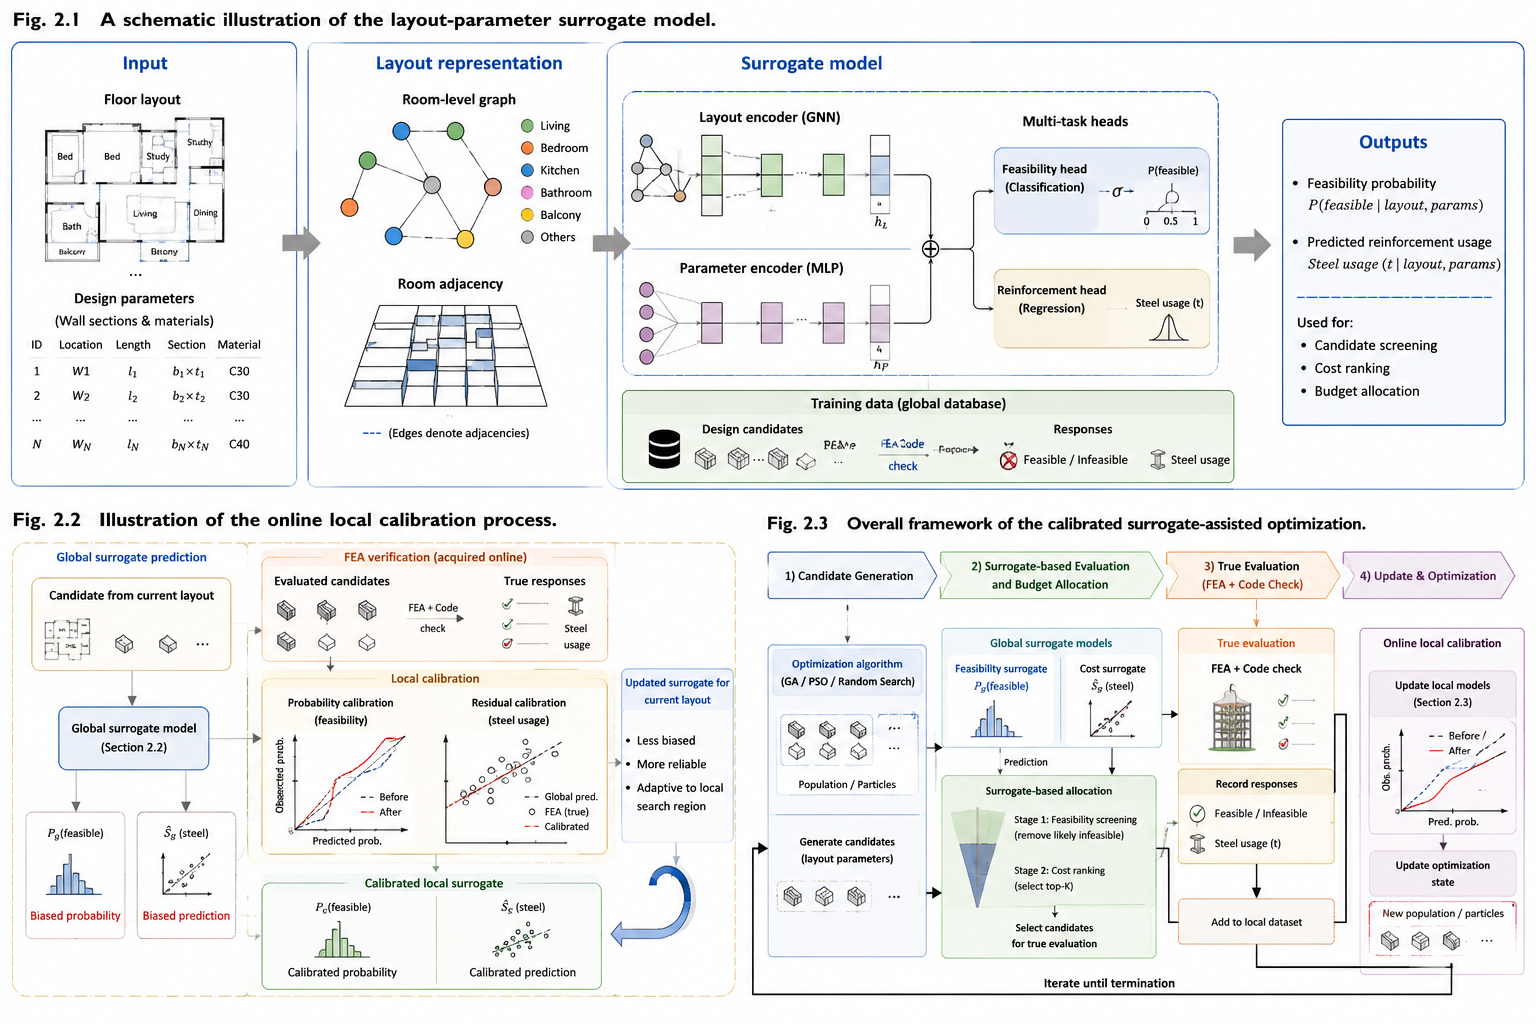
\includegraphics[width=\textwidth]{calibrated_optimization_framework.pdf}
\caption{Calibrated surrogate-assisted optimization framework.}
\label{fig:calibrated_optimization_framework}
\end{figure*}

\section{Calibrated Surrogate Modeling Method for Shear Wall Structural Optimization}
\label{sec:problem_surrogate}

To improve the efficiency of shear wall section and material optimization, the proposed method uses surrogate models to assess candidate designs before expensive FEA. In this study, true evaluation refers to the complete FEA-based workflow that generates structural responses, reinforcement design results, code-checking outcomes, and material quantities for a candidate design. A global surrogate denotes an offline model trained on FEA-verified samples from multiple layouts; it provides initial predictions of candidate feasibility and reinforcement usage. During optimization for a specific layout, candidates selected for true evaluation form a local set of newly verified samples. Online local calibration then uses this local set to correct the global surrogate predictions for the current layout. The calibrated feasibility score is used to screen clearly low-feasibility candidates, while the calibrated reinforcement prediction is used to rank promising low-cost candidates for subsequent true evaluation.

\subsection{Shear Wall Optimization Problem Formulation}
\label{subsec:expensive_problem}

For a given shear wall layout, structural optimization aims to determine suitable section and material parameters while satisfying multiple design constraints. These parameters include wall thicknesses in different vertical zones, beam section dimensions, concrete strength grades, and other design-related variables. Although the layout of the structure is fixed, different parameter combinations may lead to substantially different structural responses, reinforcement demands, and material costs.

Let $L$ denote a fixed shear wall layout and $c$ denote the corresponding design condition, including seismic intensity, site class, seismic group, load condition, and other external design requirements. The optimization variables are denoted by $x \in \mathcal{X}$, where $\mathcal{X}$ is the candidate design space formed by the allowable values of section and material parameters.

For each candidate design $(L,c,x)$, a structural evaluator $\mathcal{E}$ is required to conduct parametric modeling, FEA, structural response extraction, member design, and code-based checking\cite{GB500112010,GB500102010}. The evaluation output is written as
\begin{equation}
\mathcal{E}(L,c,x) \rightarrow (y_f,m_s,m_c,r)
\label{eq:true_evaluator}
\end{equation}
where $y_f \in \{0,1\}$ is the comprehensive feasibility label, $m_s$ and $m_c$ denote the reinforcement and concrete quantities, respectively, and $r$ represents structural response and checking indicators such as inter-story drift ratio, torsional response, axial compression ratio, shear-compression ratio, and member design results. A candidate is regarded as feasible only when the analysis is successfully completed and all major global and componet-level checks satisfy the code requirements.

The material cost of a feasible candidate is defined as
\begin{equation}
C(L,c,x)=p_s m_s(L,c,x)+p_c m_c(L,c,x)
\label{eq:material_cost}
\end{equation}
where $p_s$ and $p_c$ are the unit prices of reinforcement and concrete, respectively. In the experiments, these unit prices are determined according to current market prices. The optimization problem can therefore be formulated as
\begin{equation}
\min_{x\in\mathcal{X}} C(L,c,x),
\quad \mathrm{s.t.}\; y_f(L,c,x)=1
\label{eq:optimization_problem}
\end{equation}

The main computational difficulty lies in the repeated calls to the structural evaluator $\mathcal{E}$. In particular, reinforcement usage is difficult to estimate accurately before FEA because it depends on internal force envelopes, componet-level design, and code-based detailing requirements. Concrete quantity can be approximately obtained from geometric information and section dimensions. Therefore, this study focuses on two surrogate outputs that are most useful before FEA evaluation: (1) the probability of passing comprehensive design checks and (2) the reinforcement usage used for cost-related ranking.


\subsection{Layout-Conditioned Candidate Representation}
\label{subsec:layout_parameter_model}

The surrogate input combines layout information and design parameters. Because structural feasibility and reinforcement demand are jointly affected by the spatial layout and the design parameters, each candidate is transformed into a unified layout-conditioned representation
\begin{equation}
z=(G,d,q)
\label{eq:candidate_representation}
\end{equation}
where $G$ is the room-level graph representation of the layout, $d$ is the candidate-specific design vector formed from the design condition $c$ and the optimization variables $x$, and $q$ is the vector of global layout statistics. Thus, $z$ serves as the standard input for both surrogate tasks in this study. Fig.~\ref{fig:layout_parameter_surrogate} shows how this representation is encoded by the global surrogate models and used to predict candidate feasibility and reinforcement usage.

The first component of $z$ is the layout graph
\begin{equation}
G=(V,E)
\label{eq:layout_graph}
\end{equation}
where rooms or spatial units are treated as nodes, and adjacency relationships between rooms are treated as edges\cite{Zhao2023}. Each room node is described by a 25-dimensional feature vector that concatenates geometric descriptors and local constraint indicators. The geometric descriptors include normalized bounding-box coordinates, bounding-box size, area, and centroid, while the constraint indicators describe local buildable or wall-placement availability around the room. Each adjacency edge is assigned an 8-dimensional attribute vector that describes the spatial relationship between two neighboring rooms, including normalized shared-boundary length, shared-boundary centroid, relative direction indicators, and a boundary-orientation flag. All geometric quantities are normalized within each layout to reduce scale dependence.

The second component, $d$, encodes the seismic design condition, site information, wall and beam section parameters, concrete grade, and other candidate-level variables. The third component, $q$, supplements the graph representation with fixed-dimensional global descriptors of the whole layout. These descriptors include building scale, wall quantity, directional wall ratio, boundary wall ratio, and other geometric or topological summaries. Through this decomposition, $G$ provides local spatial organization, $q$ provides global layout context, and $d$ provides the design choices whose feasibility and cost are to be predicted.

\subsection{Global Surrogate Models and Learning Outputs}
\label{subsec:surrogate_tasks}

Given the candidate representation $z=(G,d,q)$, the global surrogate models use a layout-conditioned graph architecture to map each candidate to pre-FEA predictions. Fig.~\ref{fig:layout_parameter_surrogate}(c) shows the model architecture. The feasibility surrogate and the reinforcement surrogate are trained as two separate models with independent parameters, but they share the same input form and the same representation-learning pipeline.

The model first encodes the three components of $z$ into fixed-dimensional embeddings. The graph component $G$ is processed by a graph neural network followed by graph-level pooling, while the design vector $d$ and the global layout statistics $q$ are mapped by separate tabular encoders. The three embeddings are then concatenated into a fused candidate representation $h$. This representation is used by the separately trained feasibility and reinforcement surrogate models to produce their respective predictions.

Based on $h$, the feasibility surrogate outputs the probability that the candidate can pass the comprehensive structural checks:
\begin{equation}
\hat{p}_{f}^{G}=\sigma(f_{\theta_f}(h))
\label{eq:feasibility_output}
\end{equation}
where $\sigma(\cdot)$ is the sigmoid function and $\hat{p}_{f}^{G}\in[0,1]$. This output is used as a conservative screening score. Candidates with very low predicted feasibility can be assigned low priority, while potentially feasible candidates are retained for further ranking or true evaluation.

The reinforcement surrogate outputs the predicted reinforcement usage:
\begin{equation}
\hat{m}_{s}^{G}=f_{\theta_s}(h)
\label{eq:steel_output}
\end{equation}

This output is used as the cost-related ranking signal before FEA. Since concrete quantity can be rapidly approximated from geometry and section dimensions, the global surrogate cost estimate is written as
\begin{equation}
\hat{C}^{G}=p_s\hat{m}_{s}^{G}+p_c\tilde{m}_c
\label{eq:global_surrogate_cost}
\end{equation}
where $\tilde{m}_c$ is the estimated concrete quantity. Candidates with lower surrogate cost are assigned higher priority for true FEA evaluation after feasibility screening.

The two surrogate models are trained with task-specific losses. The feasibility model is optimized using a weighted binary cross-entropy loss to account for class imbalance:
\begin{equation}
\mathcal{L}_f = -\omega y_f \log \hat{p}_{f}^{G} - (1-y_f)\log(1-\hat{p}_{f}^{G})
\label{eq:feasibility_loss}
\end{equation}
where $\omega$ is the class weight. For reinforcement prediction, the target $m_s$ is first transformed using logarithmic scaling and standardization:
\begin{equation}
y_s=\frac{\log(1+m_s)-\mu_s}{\sigma_s}
\label{eq:steel_transform}
\end{equation}
where $\mu_s$ and $\sigma_s$ are computed from the training set. The reinforcement surrogate is trained using the Smooth L1 loss in the transformed space\cite{Huber1964}:
\begin{equation}
\mathcal{L}_s=\frac{1}{N_s}\sum_{i=1}^{N_s}\rho_\beta(e_i),
\quad e_i=\hat{y}_{s,i}-y_{s,i}
\label{eq:steel_loss}
\end{equation}
\begin{equation}
\rho_\beta(e_i)=
\begin{cases}
\dfrac{e_i^2}{2\beta}, & |e_i|<\beta, \\
|e_i|-\dfrac{\beta}{2}, & |e_i|\ge\beta
\end{cases}
\label{eq:smooth_l1}
\end{equation}
where $N_s$ is the number of reinforcement training samples and $\beta$ controls the transition between the quadratic and linear penalty regions. During inference, the predicted reinforcement usage is recovered by applying the inverse transformation of Eqn.~\ref{eq:steel_transform}.

\subsection{Online Local Calibration of Global Surrogates}
\label{subsec:online_local_calibration}

A global surrogate trained on multiple layouts provides useful prior knowledge for unseen design cases, but it may still exhibit systematic bias for a particular layout or local search region. This issue is especially important in shear wall optimization because the candidate distribution of design variable changes during the search. Therefore, using a static global surrogate throughout the optimization process may lead to inappropriate screening or ranking decisions.

To address this problem, this study introduces online local calibration. 
Fig.~\ref{fig:online_calibration} illustrates the online local calibration process.
During optimization, candidates selected for true evaluation naturally produce FEA-verified samples. These samples are accumulated as a local calibration set:
\begin{equation}
\mathcal{D}_{t}^{loc}
=
\left\{
(z_i,\hat{p}_{f,i}^{G},\hat{m}_{s,i}^{G},y_{f,i},m_{s,i})
\right\}_{i=1}^{n_t}
\label{eq:local_dataset}
\end{equation}
where $t$ denotes the current optimization iteration and $n_t$ is the number of locally verified samples. The local set stores both global surrogate predictions and true FEA-based ground truth, enabling the calibration module to learn the prediction bias of the global surrogate under the current layout.

\subsubsection{Feasibility probability calibration}
\label{subsubsec:feasibility_calibration}

For feasibility prediction, the goal of calibration is to adjust the global surrogate probability so that it better reflects the observed feasible rate in the current layout and local search region\cite{Zadrozny2002}. The global probability is first converted into a logit value:
\begin{equation}
\ell^{G}
=
\log
\frac{\hat{p}_{f}^{G}}{1-\hat{p}_{f}^{G}}
\label{eq:global_logit}
\end{equation}

When the local calibration set contains enough samples and both feasible and infeasible cases, a lightweight calibration function $g_t(\cdot)$ is fitted:
\begin{equation}
\hat{p}_{f}^{C}=g_t(\ell^{G})
\label{eq:calibrated_probability}
\end{equation}
where $\hat{p}_{f}^{C}$ is the calibrated feasibility probability.

This calibration adjusts the global feasibility probability $\hat{p}_{f}^{G}$ into a layout-specific feasibility score $\hat{p}_{f}^{C}$. The calibrated score is then used for candidate screening in the current layout. To keep the screening conservative, the threshold is chosen from locally verified feasible samples. Given a target recall $r_0$ for feasible candidates, the raw threshold is defined as
\begin{equation}
\tau_t^{raw}
=
Q_{1-r_0}
\left(
\left\{
\hat{p}_{f}^{C}\mid y_{f}=1
\right\}
\right)
\label{eq:raw_threshold}
\end{equation}
where $Q_{1-r_0}(\cdot)$ denotes the quantile function. A conservative scaling coefficient $\alpha\in(0,1]$ is then applied:
\begin{equation}
\tau_t^{C}=\alpha \tau_t^{raw}
\label{eq:calibrated_threshold}
\end{equation}

A candidate with $\hat{p}_{f}^{C}<\tau_t^{C}$ is regarded as low priority for true FEA evaluation. If there are no enough local samples for calibration, the framework falls back to the global feasibility probability and a validation-based global threshold.

\subsubsection{Reinforcement residual calibration}
\label{subsubsec:steel_calibration}

For reinforcement usage, the main purpose of calibration is to correct the systematic residual between the global surrogate prediction and the true reinforcement quantity. For a locally verified sample, the residual is defined as
\begin{equation}
\Delta m_{s}
=
m_{s}-\hat{m}_{s}^{G}
\label{eq:steel_residual}
\end{equation}

A local residual model $r_t(\cdot)$ is fitted using the local calibration set:
\begin{equation}
\widehat{\Delta m}_{s}=r_t(z,\hat{m}_{s}^{G})
\label{eq:residual_model}
\end{equation}

The calibrated reinforcement prediction is then obtained by
\begin{equation}
\hat{m}_{s}^{C}
=
\hat{m}_{s}^{G}
+
\widehat{\Delta m}_{s}
\label{eq:calibrated_steel}
\end{equation}

Compared with retraining the full graph surrogate model, this residual calibration strategy is lightweight and sample-efficient. The global surrogate captures the overall mapping learned from multiple layouts, while the local residual model only needs to correct the remaining layout-specific bias. The calibrated reinforcement prediction can be combined with the estimated concrete quantity to form a calibrated surrogate cost:
\begin{equation}
\hat{C}^{C}
=
p_s\hat{m}_{s}^{C}
+
p_c\tilde{m}_{c}
\label{eq:calibrated_cost}
\end{equation}
This calibrated cost estimate is used for candidate ranking before true evaluation.
 % related works


\begin{figure*}[t]
\centering
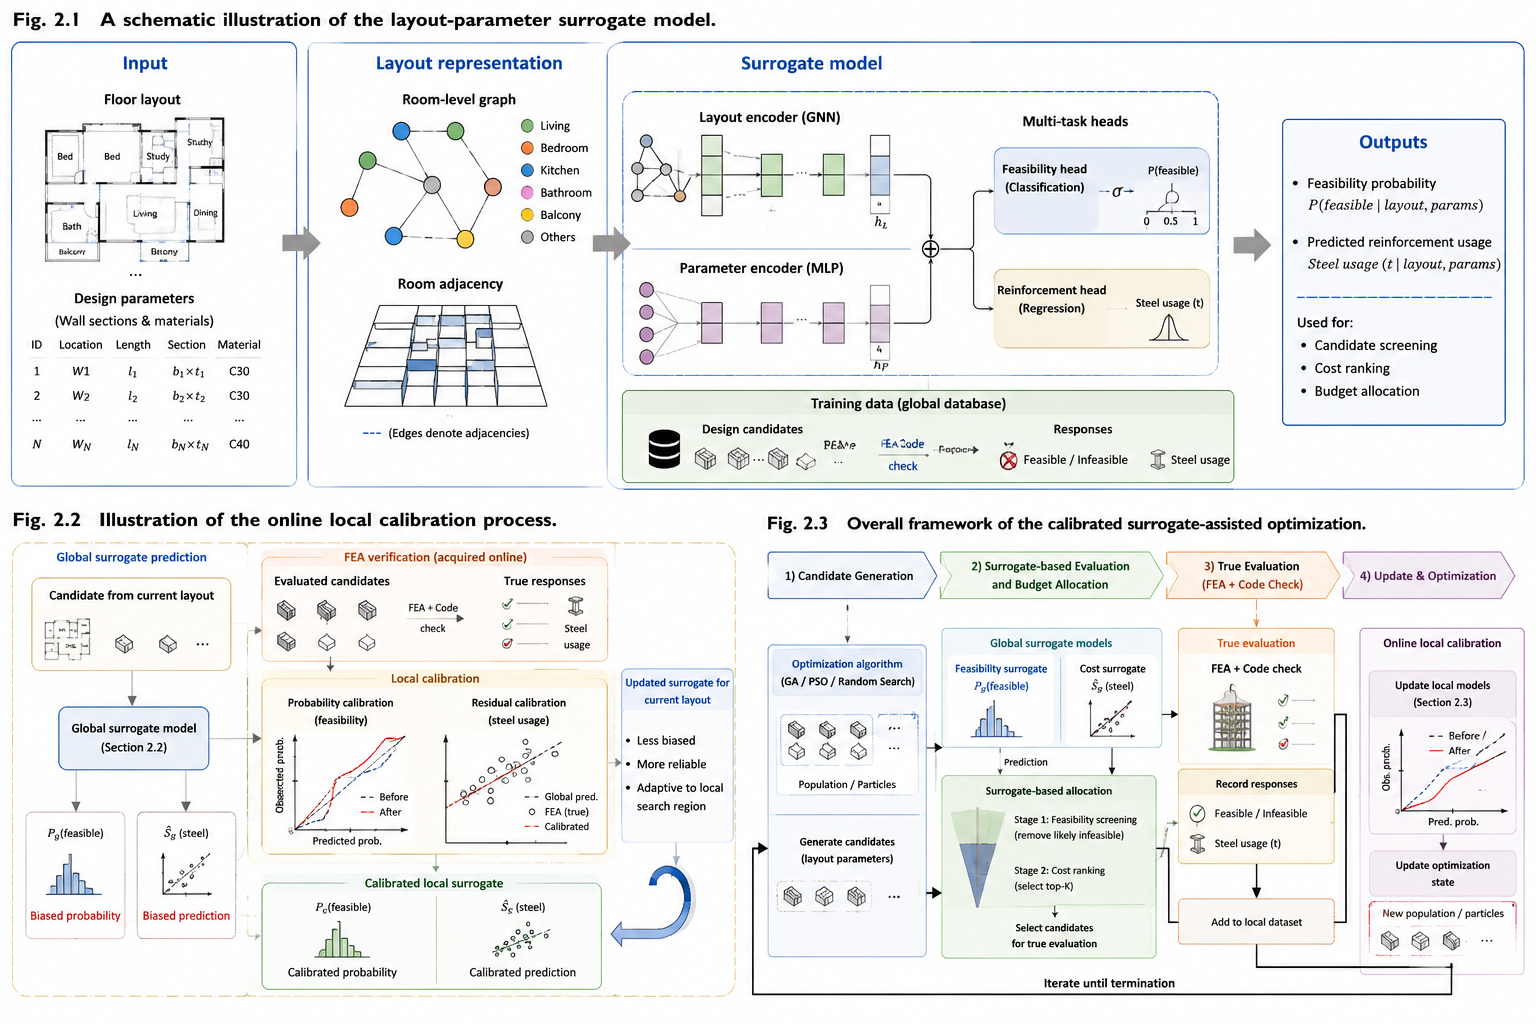
\includegraphics[width=\textwidth]{calibrated_optimization_framework.png}
\caption{Calibrated surrogate-assisted optimization framework.}
\label{fig:calibrated_optimization_framework}
\end{figure*}

\section{Calibrated Surrogate-Assisted Optimization Framework}
\label{sec:optimization_framework}

This section further describes how these models are embedded into an optimization process. 

\subsection{Overall Framework}
\label{subsec:overall_framework}

The overall framework is illustrated in Fig.~\ref{fig:calibrated_optimization_framework}. For a fixed shear wall layout $L$ and design condition $c$, the optimization task is to search the design space $\mathcal{X}$ for section and material parameters that minimize the material cost while satisfying all structural checks. At iteration $t$, the optimizer $\mathcal{O}$ generates a batch of candidate designs:
\begin{equation}
\mathcal{B}_t=
\left\{
x_{t,1},x_{t,2},\ldots,x_{t,N_b}
\right\},
\label{eq:candidate_batch}
\end{equation}
where $N_b$ is the batch size.

For each candidate $x_{t,i}$, the corresponding input representation is constructed as a structured tuple:
\begin{equation}
z_{t,i}=\left(G,q,d_{t,i}\right),
\label{eq:candidate_input_framework}
\end{equation}
where $G$ is the room-level layout graph, $q$ is the vector of global layout statistics, and $d_{t,i}$ is the design-parameter vector formed by $x_{t,i}$ and the design condition $c$. This notation indicates that graph features, global layout statistics, and design parameters are passed to the surrogate model as separate input components and fused inside the model. Since the layout and design condition remain fixed in a single optimization task, $G$ and $q$ are constant, while $d_{t,i}$ varies among candidates.

The global surrogate models first provide feasibility and reinforcement predictions for all candidates:
\begin{equation}
\hat{p}_{f,t,i}^{G}=SM_f(z_{t,i}),
\label{eq:global_feasibility_framework}
\end{equation}
\begin{equation}
\hat{m}_{s,t,i}^{G}=SM_s(z_{t,i}).
\label{eq:global_steel_framework}
\end{equation}
If the local calibration set $\mathcal{D}_{t}^{loc}$ contains enough verified samples to fit the calibration models, the global predictions are corrected by the online calibration module:
\begin{equation}
\hat{p}_{f,t,i}^{C}=\mathcal{C}_{f,t}(\hat{p}_{f,t,i}^{G}),
\label{eq:calibrated_feasibility_framework}
\end{equation}
\begin{equation}
\hat{m}_{s,t,i}^{C}=\mathcal{C}_{s,t}(z_{t,i},\hat{m}_{s,t,i}^{G}),
\label{eq:calibrated_steel_framework}
\end{equation}
where $\mathcal{C}_{f,t}$ and $\mathcal{C}_{s,t}$ denote the feasibility probability calibration model and the reinforcement residual calibration model at iteration $t$, respectively.

The calibrated predictions are then used for candidate screening and priority ranking. The candidate subset selected for true evaluation is denoted by $\mathcal{S}_t\subseteq \mathcal{B}_t$. For each candidate in $\mathcal{S}_t$, the true evaluator produces FEA-verified results:
\begin{equation}
\mathcal{E}(L,c,x_{t,i})
\rightarrow
(y_{f,t,i},m_{s,t,i},m_{c,t,i},r_{t,i}),
\quad x_{t,i}\in\mathcal{S}_t .
\label{eq:true_eval_framework}
\end{equation}
These verified results are used to update the optimizer and to expand the local calibration set.

\subsection{Candidate Screening and Priority Ranking}
\label{subsec:candidate_screening_ranking}

The surrogate-based pre-evaluation module consists of two consecutive operations, feasibility screening and priority ranking. The first operation aims to reduce unnecessary FEA calls for candidates that are very unlikely to satisfy the structural checks. The second operation prioritizes candidates that are more likely to achieve low material cost under the limited FEA budget.

Given the calibrated feasibility probability $\hat{p}_{f,t,i}^{C}$ and the screening threshold $\tau_t$, the candidates passing the feasibility screening are defined as
\begin{equation}
\mathcal{B}_{t}^{pass}
=
\left\{
x_{t,i}\in\mathcal{B}_t
\mid
\hat{p}_{f,t,i}^{C}\ge \tau_t
\right\}.
\label{eq:pass_set}
\end{equation}
The threshold $\tau_t$ follows the conservative strategy introduced in Section~\ref{subsec:online_local_calibration}. Its purpose is to avoid removing potentially feasible designs.

Because the optimizers minimize a scalar objective value, candidates that are not submitted to FEA still need a placeholder fitness for optimizer bookkeeping. These candidates, including those rejected by screening or skipped after ranking, are assigned a large rejected objective:
\begin{equation}
F^{rej}(x_{t,i}) = M_{rej},
\quad M_{rej}=1.0\times 10^{12}.
\label{eq:rejected_objective}
\end{equation}
This value is much larger than normal material-cost or penalty values, so such candidates are dominated in the minimization process and are effectively skipped by the optimizer. The rejected objective is not a verified infeasibility label and is not used for best-solution comparison or local calibration.

For a truly evaluated candidate design ${x}_{t,i}$, the scalar fitness used by the optimizer is defined as
\begin{equation}
F({x}_{t,i})
=
\begin{cases}
C({x}_{t,i}), 
& {x}_{t,i}\in\Omega_f,\\[3pt]
P_0+\lambda_v V({x}_{t,i})+\lambda_c C({x}_{t,i}),
& {x}_{t,i}\notin\Omega_f,
\end{cases}
\label{eq:true_fitness}
\end{equation}
where $C({x}_{t,i})$ is the material cost, $\Omega_f$ denotes the feasible domain, $P_0$ is a base infeasibility penalty, and $\lambda_v$ and $\lambda_c$ are the violation and cost weights for infeasible candidates. The violation measure is
\begin{equation}
\begin{aligned}
V({x}_{t,i})
={}&
\sum_{r}
\max\left(
0,
\frac{g_r({x}_{t,i})-g_r^{\lim}}{g_r^{\lim}}
\right) \\
&+
\sum_{s}
\max\left(
0,
\frac{h_s^{\lim}-h_s({x}_{t,i})}{h_s^{\lim}}
\right) \\
&+
\sum_{q} b_q({x}_{t,i}),
\end{aligned}
\label{eq:violation_score}
\end{equation}
where $g_r$ denotes upper-bound constraints, $h_s$ denotes lower-bound constraints, and $b_q\in\{0,1\}$ indicates whether a discrete code-check item fails. Therefore, infeasible candidates are primarily ranked by their degree of code violation, while feasible candidates are ranked directly by material cost.


For a candidate that is not rejected by the feasibility screener, The surrogate ranking score is then defined as
\begin{equation}
S_{t,i}^{C}
=
\hat{C}_{t,i}^{C}
+
\eta
\max(0,p_0-\hat{p}_{f,t,i}^{C}),
\label{eq:ranking_score}
\end{equation}
where $\hat{p}_{f,t,i}^{C}$ is the calibrated feasibility probability, $p_0$ is the feasibility hinge threshold, and $\eta$ is the risk-penalty coefficient.


The FEA budget at iteration $t$ is adaptive. Before any feasible design has been observed, a larger budget is used:
\begin{equation}
K_t^{pre}
=
\max
\left(
K_{\min},
\left\lceil r_{pre}|\mathcal{B}_t^{pass}|\right\rceil
\right),
\label{eq:pre_feasible_budget}
\end{equation}
where $r_{pre}=0.8$ in the experiments. The selected set is obtained by the lowest surrogate scores:
\begin{equation}
\mathcal{S}_t
=
\mathrm{TopK}
\left(
\mathcal{B}_t^{pass}, S_{t,i}^{C}, K_t^{pre}
\right).
\label{eq:pre_feasible_selection}
\end{equation}

After at least one feasible design has been found, the selection switches to a mixed strategy:
\begin{equation}
K_t
=
\max
\left(
K_{\min},
\left\lceil r|\mathcal{B}_t^{pass}|\right\rceil
\right),
\label{eq:post_feasible_budget}
\end{equation}
and
\begin{equation}
\mathcal{S}_t
=
\mathcal{S}_t^{cost}
\cup
\mathcal{S}_t^{risk}
\cup
\mathcal{S}_t^{div},
\label{eq:mixed_selection}
\end{equation}
where $\mathcal{S}_t^{cost}$ contains the candidates with the lowest surrogate cost scores, $\mathcal{S}_t^{risk}$ contains candidates with the lowest feasibility risk, and $\mathcal{S}_t^{div}$ is a randomly sampled exploration subset. In the experiments, the three quotas are set to 60\%, 25\%, and 15\% of $K_t$, respectively. If the union contains fewer than $K_t$ candidates, the remaining budget is filled by the lowest-score candidates not yet selected.



Through this two-stage mechanism, the feasibility surrogate and the reinforcement surrogate have different but complementary functions. The feasibility surrogate reduces the probability that clearly infeasible candidates consume FEA calls, whereas the reinforcement surrogate ranks the remaining candidates by material economy. Online local calibration improves both decisions by adapting the global surrogate predictions to the current layout and search region.

\subsection{Online Update with FEA-Verified Samples}
\label{subsec:online_update_framework}

After the selected candidates $\mathcal{S}_t$ are evaluated by the true evaluator, their verified results are used in two ways. First, they are used by the optimizer to update the search state. For a feasible candidate, the true material cost is calculated from the verified reinforcement and concrete quantities:
\begin{equation}
C_{t,i}
=
\pi_s m_{s,t,i}
+
\pi_c m_{c,t,i},
\quad y_{f,t,i}=1 .
\label{eq:true_cost_framework}
\end{equation}
This value is used as the true objective value for optimizer update and best-solution comparison. Infeasible candidates are handled according to the constraint-handling strategy of the optimizer.

Second, the same verified samples are added to the local calibration set:
\begin{equation}
\begin{aligned}
\mathcal{D}_{t+1}^{loc}
=
\mathcal{D}_{t}^{loc}
\cup
\bigl\{
&(z_{t,i},
\hat{p}_{f,t,i}^{G},
\hat{m}_{s,t,i}^{G},
y_{f,t,i},
m_{s,t,i})
&\mid x_{t,i}\in\mathcal{S}_t
\bigr\}.
\end{aligned}
\label{eq:local_set_update}
\end{equation}
The stored global predictions and verified labels allow the calibration module to learn layout-specific probability shifts and reinforcement residuals. Candidates that are not evaluated by FEA have no verified labels and are therefore not used for calibration.

At the beginning of optimization, $\mathcal{D}_{t}^{loc}$ may be empty or too small for reliable calibration, and the framework mainly relies on global surrogate predictions with conservative screening. As more FEA-verified samples are accumulated, the local calibration module becomes active and progressively corrects the global surrogate bias. This online update process allows the surrogate module to become more consistent with the current optimization task without retraining the full global graph model.

\subsection{Algorithm Summary}
\label{subsec:algorithm_summary}

The complete calibrated surrogate-assisted optimization procedure is summarized in Algorithm~\ref{alg:csa_optimization}. The algorithm takes a fixed layout, design condition, design space, optimizer, global surrogate models, true evaluator, rejected objective, and FEA budget as inputs. It outputs the best feasible design found within the FEA budget.

\begin{algorithm}[t]
\caption{Calibrated surrogate-assisted optimization}
\label{alg:csa_optimization}
\begin{algorithmic}[1]
\REQUIRE Layout $L$, design condition $c$, design space $\mathcal{X}$, optimizer $\mathcal{O}$, global surrogates $SM_f$ and $SM_s$, true evaluator $\mathcal{E}$, rejected objective $M_{rej}$, initial local calibration set $\mathcal{D}_{0}^{loc}=\emptyset$, FEA budget.
\ENSURE Best feasible design verified by $\mathcal{E}$.
\FOR{$t=0,1,\ldots,T-1$}
\STATE Generate a candidate batch $\mathcal{B}_t$ using optimizer $\mathcal{O}$.
\STATE Construct candidate representations $z_{t,i}=\left(G,q,d_{t,i}\right)$ for all $x_{t,i}\in\mathcal{B}_t$.
\STATE Obtain global predictions $\hat{p}_{f,t,i}^{G}=SM_f(z_{t,i})$ and $\hat{m}_{s,t,i}^{G}=SM_s(z_{t,i})$.
\IF{$\mathcal{D}_{t}^{loc}$ contains enough verified samples for calibration}
\STATE Compute calibrated predictions $\hat{p}_{f,t,i}^{C}$ and $\hat{m}_{s,t,i}^{C}$.
\ELSE
\STATE Set $\hat{p}_{f,t,i}^{C}=\hat{p}_{f,t,i}^{G}$ and $\hat{m}_{s,t,i}^{C}=\hat{m}_{s,t,i}^{G}$.
\ENDIF
\STATE Screen candidates according to $\hat{p}_{f,t,i}^{C}$ and $\tau_t$.
\STATE Rank the retained candidates using the score $S_{t,i}^{C}$.
\STATE Select $\mathcal{S}_t$ for true FEA and code-based checking.
\STATE Evaluate each $x_{t,i}\in\mathcal{S}_t$ using $\mathcal{E}$ to obtain $(y_{f,t,i},m_{s,t,i},m_{c,t,i},r_{t,i})$.
\STATE Assign $M_{rej}$ to candidates in $\mathcal{B}_t\setminus\mathcal{S}_t$.
\STATE Update optimizer $\mathcal{O}$ using FEA-verified results and rejected-objective values.
\STATE Update the local calibration set $\mathcal{D}_{t+1}^{loc}$.
\ENDFOR
\STATE \RETURN The best feasible design verified by $\mathcal{E}$.
\end{algorithmic}
\end{algorithm}

The proposed algorithm keeps the true structural evaluator as the only source of verified feasibility and objective values. The surrogate module only changes how candidate designs are prioritized before evaluation. % methodology

\section{Experimental Setup}
\label{sec:experimental_setup}

This section describes the experimental design used to evaluate three key components of the proposed calibrated surrogate-assisted optimization framework.

\subsection{Experimental Objectives}
\label{subsec:experimental_objectives}

First, the global surrogate models are evaluated on unseen shear wall layouts. The feasibility surrogate is assessed in terms of both classification performance and conservative screening ability, while the reinforcement surrogate is assessed in terms of prediction accuracy and ranking quality. To verify the role of layout representation, three input settings are compared: design parameters only, design parameters with global layout statistics, and the proposed graph-based layout representation.

Second, the effectiveness of online local calibration is investigated. Since each optimization task is performed for a fixed layout and design condition, FEA-verified samples generated during optimization can provide layout-specific feedback. The calibration experiments therefore examine whether a small number of locally verified samples can improve feasibility probability calibration, reduce reinforcement prediction bias, and improve candidate ranking in the current layout.

Third, the calibrated surrogate models are embedded into optimization procedures. The optimization experiments compare full FEA-based optimization with several surrogate-assisted evaluation strategies. The comparison focuses on the number of true FEA calls, feasible-solution discovery, and final material cost. All compared methods use the same design space and true evaluator.

\begin{table}[t]
\centering
\caption{Sampling space of structural design parameters.}
\label{tab:parameter_space}
\setlength{\tabcolsep}{3pt}
\begin{tabularx}{\columnwidth}{@{}>{\raggedright\arraybackslash}p{0.30\columnwidth}>{\centering\arraybackslash}p{0.17\columnwidth}>{\centering\arraybackslash}p{0.08\columnwidth}>{\raggedright\arraybackslash}X@{}}
\toprule
Parameter & Symbol & Unit & Sampling values \\
\midrule
Number of stories & $N$ & - & 18--33 \\
Story height & $h_{story}$ & m & 2.9 \\
Bottom wall thickness & $t_{w,b}$ & mm & 200, 250, 300, 350, 400 \\
Middle wall thickness & $t_{w,m}$ & mm & 160, 180, 200, 250, 300 \\
Top wall thickness & $t_{w,t}$ & mm & 160, 180, 200, 250 \\
Main beam depth & $h_{m}$ & mm & 400, 500, 550, 600, 650, 700 \\
Main beam width & $b_{m}$ & mm & 200, 250, 300, 350 \\
Secondary beam depth & $h_{s}$ & mm & 300, 400, 450, 500 \\
Secondary beam width & $b_{s}$ & mm & 200, 250, 300 \\
Concrete grade & $f_c$ & - & C30, C35, C40, C45, C50 \\
Seismic intensity & $S_I$ & - & 6.0, 7.0, 7.5, 8.0 \\
Site class & $S_C$ & - & I0, I, II, III, IV \\
Seismic group & $S_G$ & - & 1, 2, 3 \\
\bottomrule
\end{tabularx}
\end{table}

\begin{table*}[t]
\centering
\caption{Dataset split and design-condition groups.}
\label{tab:dataset_split}
\setlength{\tabcolsep}{5pt}
\begin{tabularx}{\textwidth}{@{}>{\raggedright\arraybackslash}p{0.18\textwidth}
>{\centering\arraybackslash}p{0.15\textwidth}
>{\centering\arraybackslash}p{0.16\textwidth}
>{\centering\arraybackslash}X@{}}
\toprule
Subset & No. of layouts & No. of samples & Group ratio (Group7-H1 / Group7-H2 / Group8) \\
\midrule
Training & 100 & 499,977 & 19.0\% / 38.0\% / 43.0\% \\
Validation & 22  & 109,996 & 33.3\% / 47.6\% / 19.0\% \\
Testing & 21 & 104,999 & 31.8\% / 18.2\% / 50.0\% \\
\midrule
Total & 143 & 714,972 & 23.1\% / 36.4\% / 40.6\% \\
\bottomrule
\end{tabularx}
\end{table*}


\begin{figure*}[t]
\centering
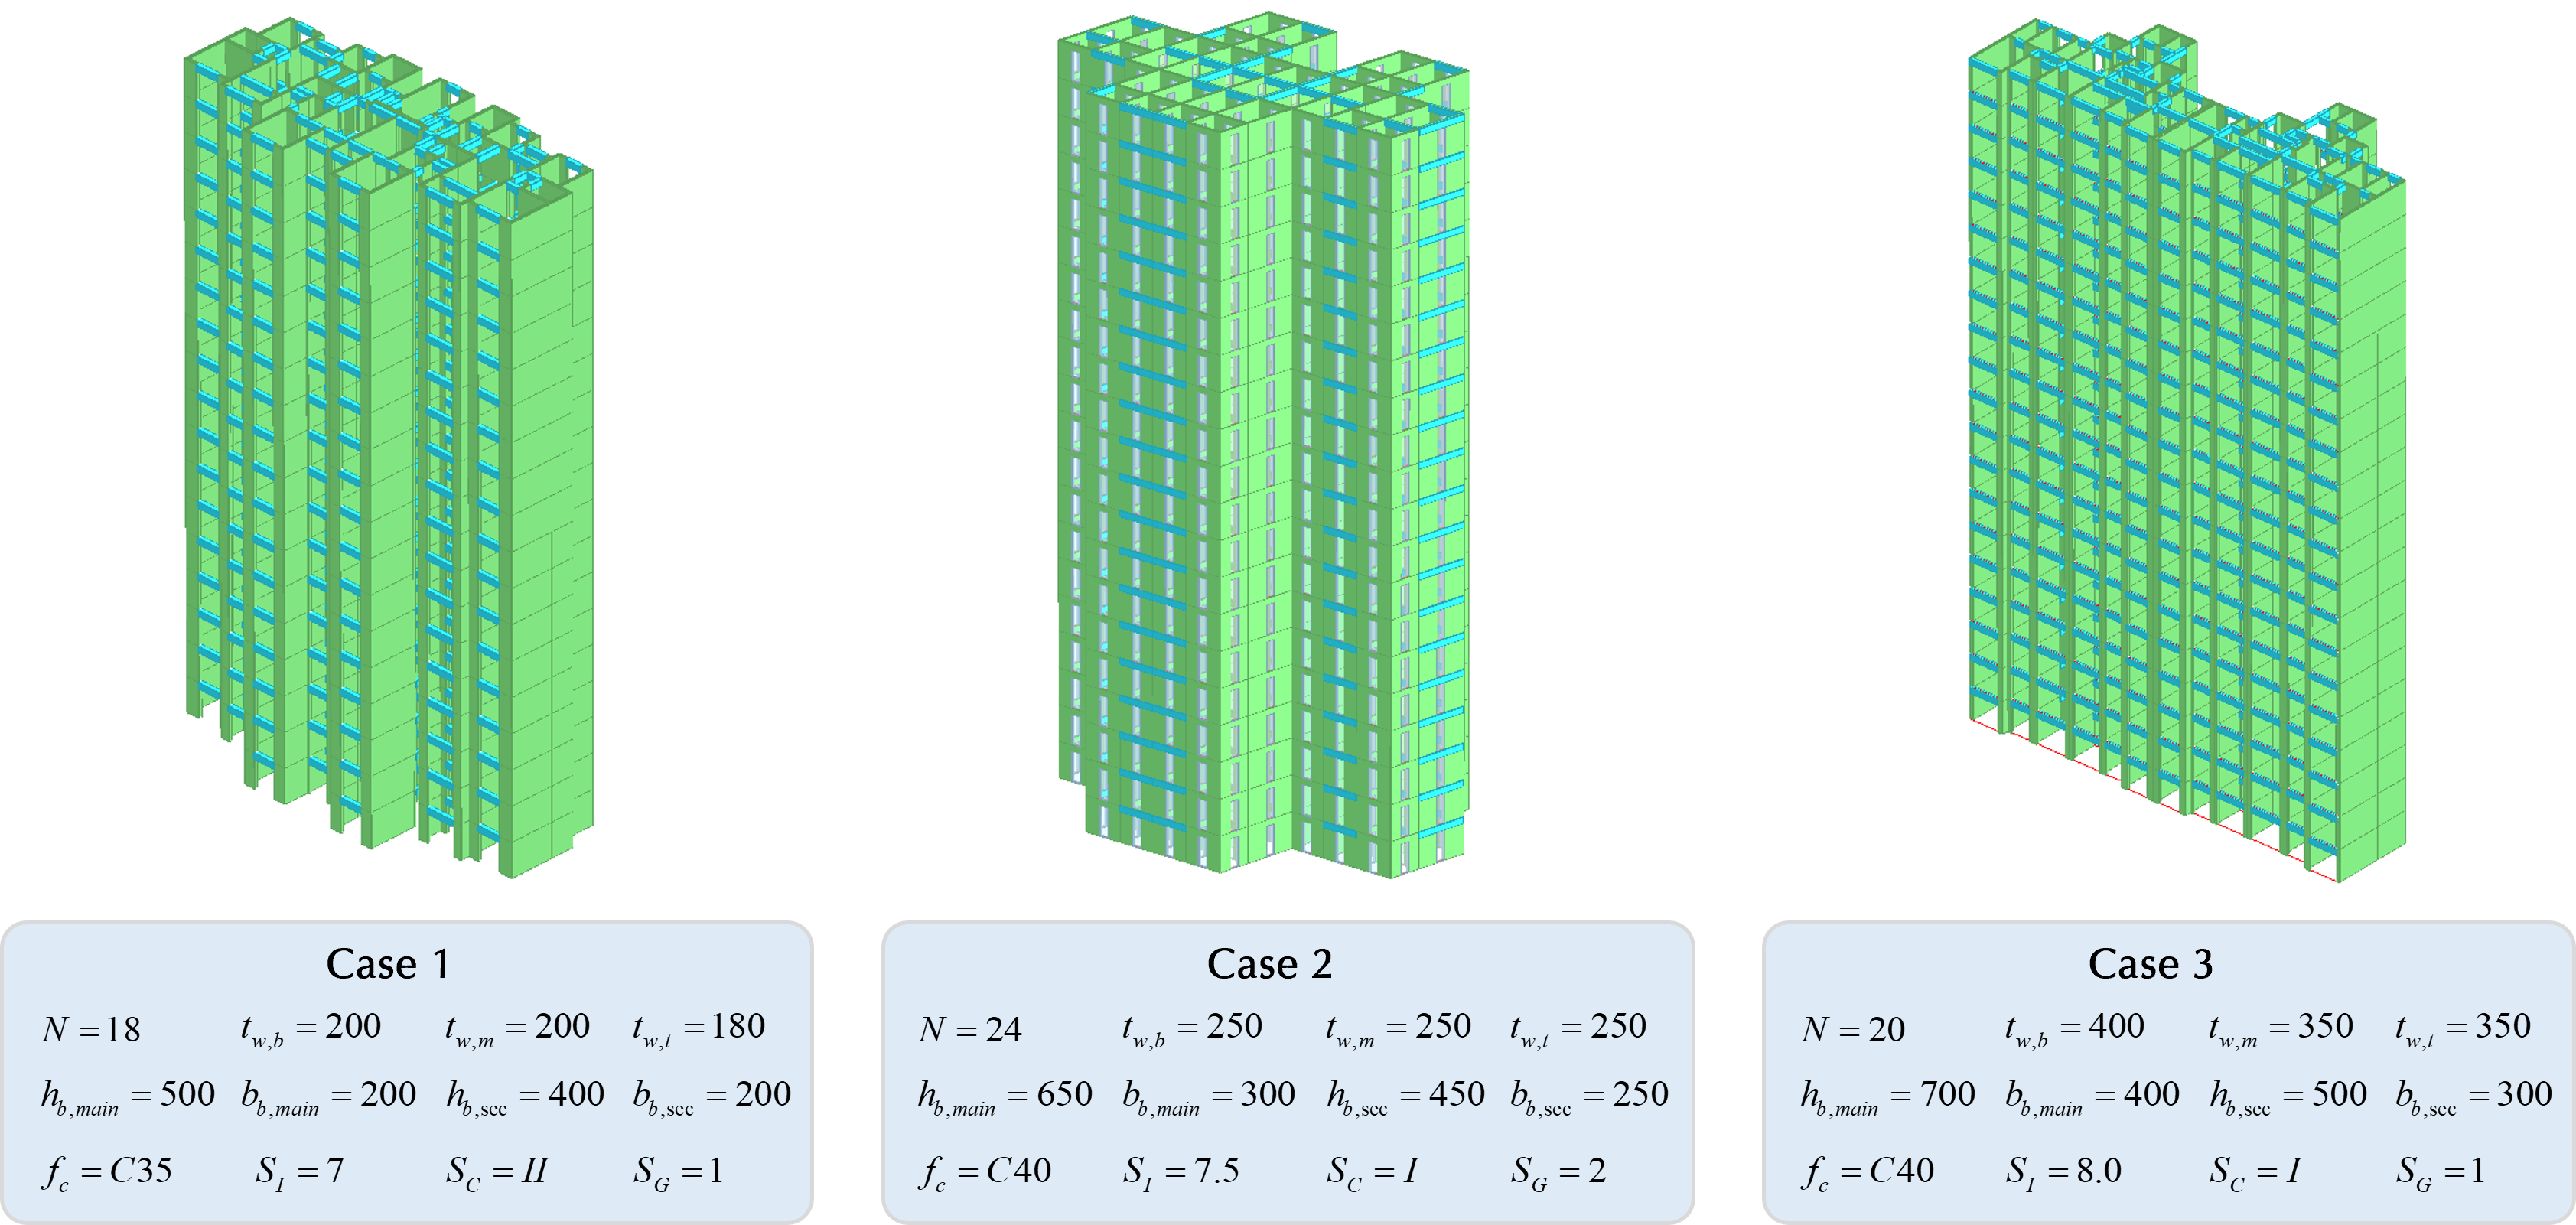
\includegraphics[width=\textwidth]{model_cases.png}
\caption{Representative finite element models of shear wall structures under different sampled design parameters and design conditions.}
\label{fig:model_cases}
\end{figure*}


\begin{figure*}[t]
\centering
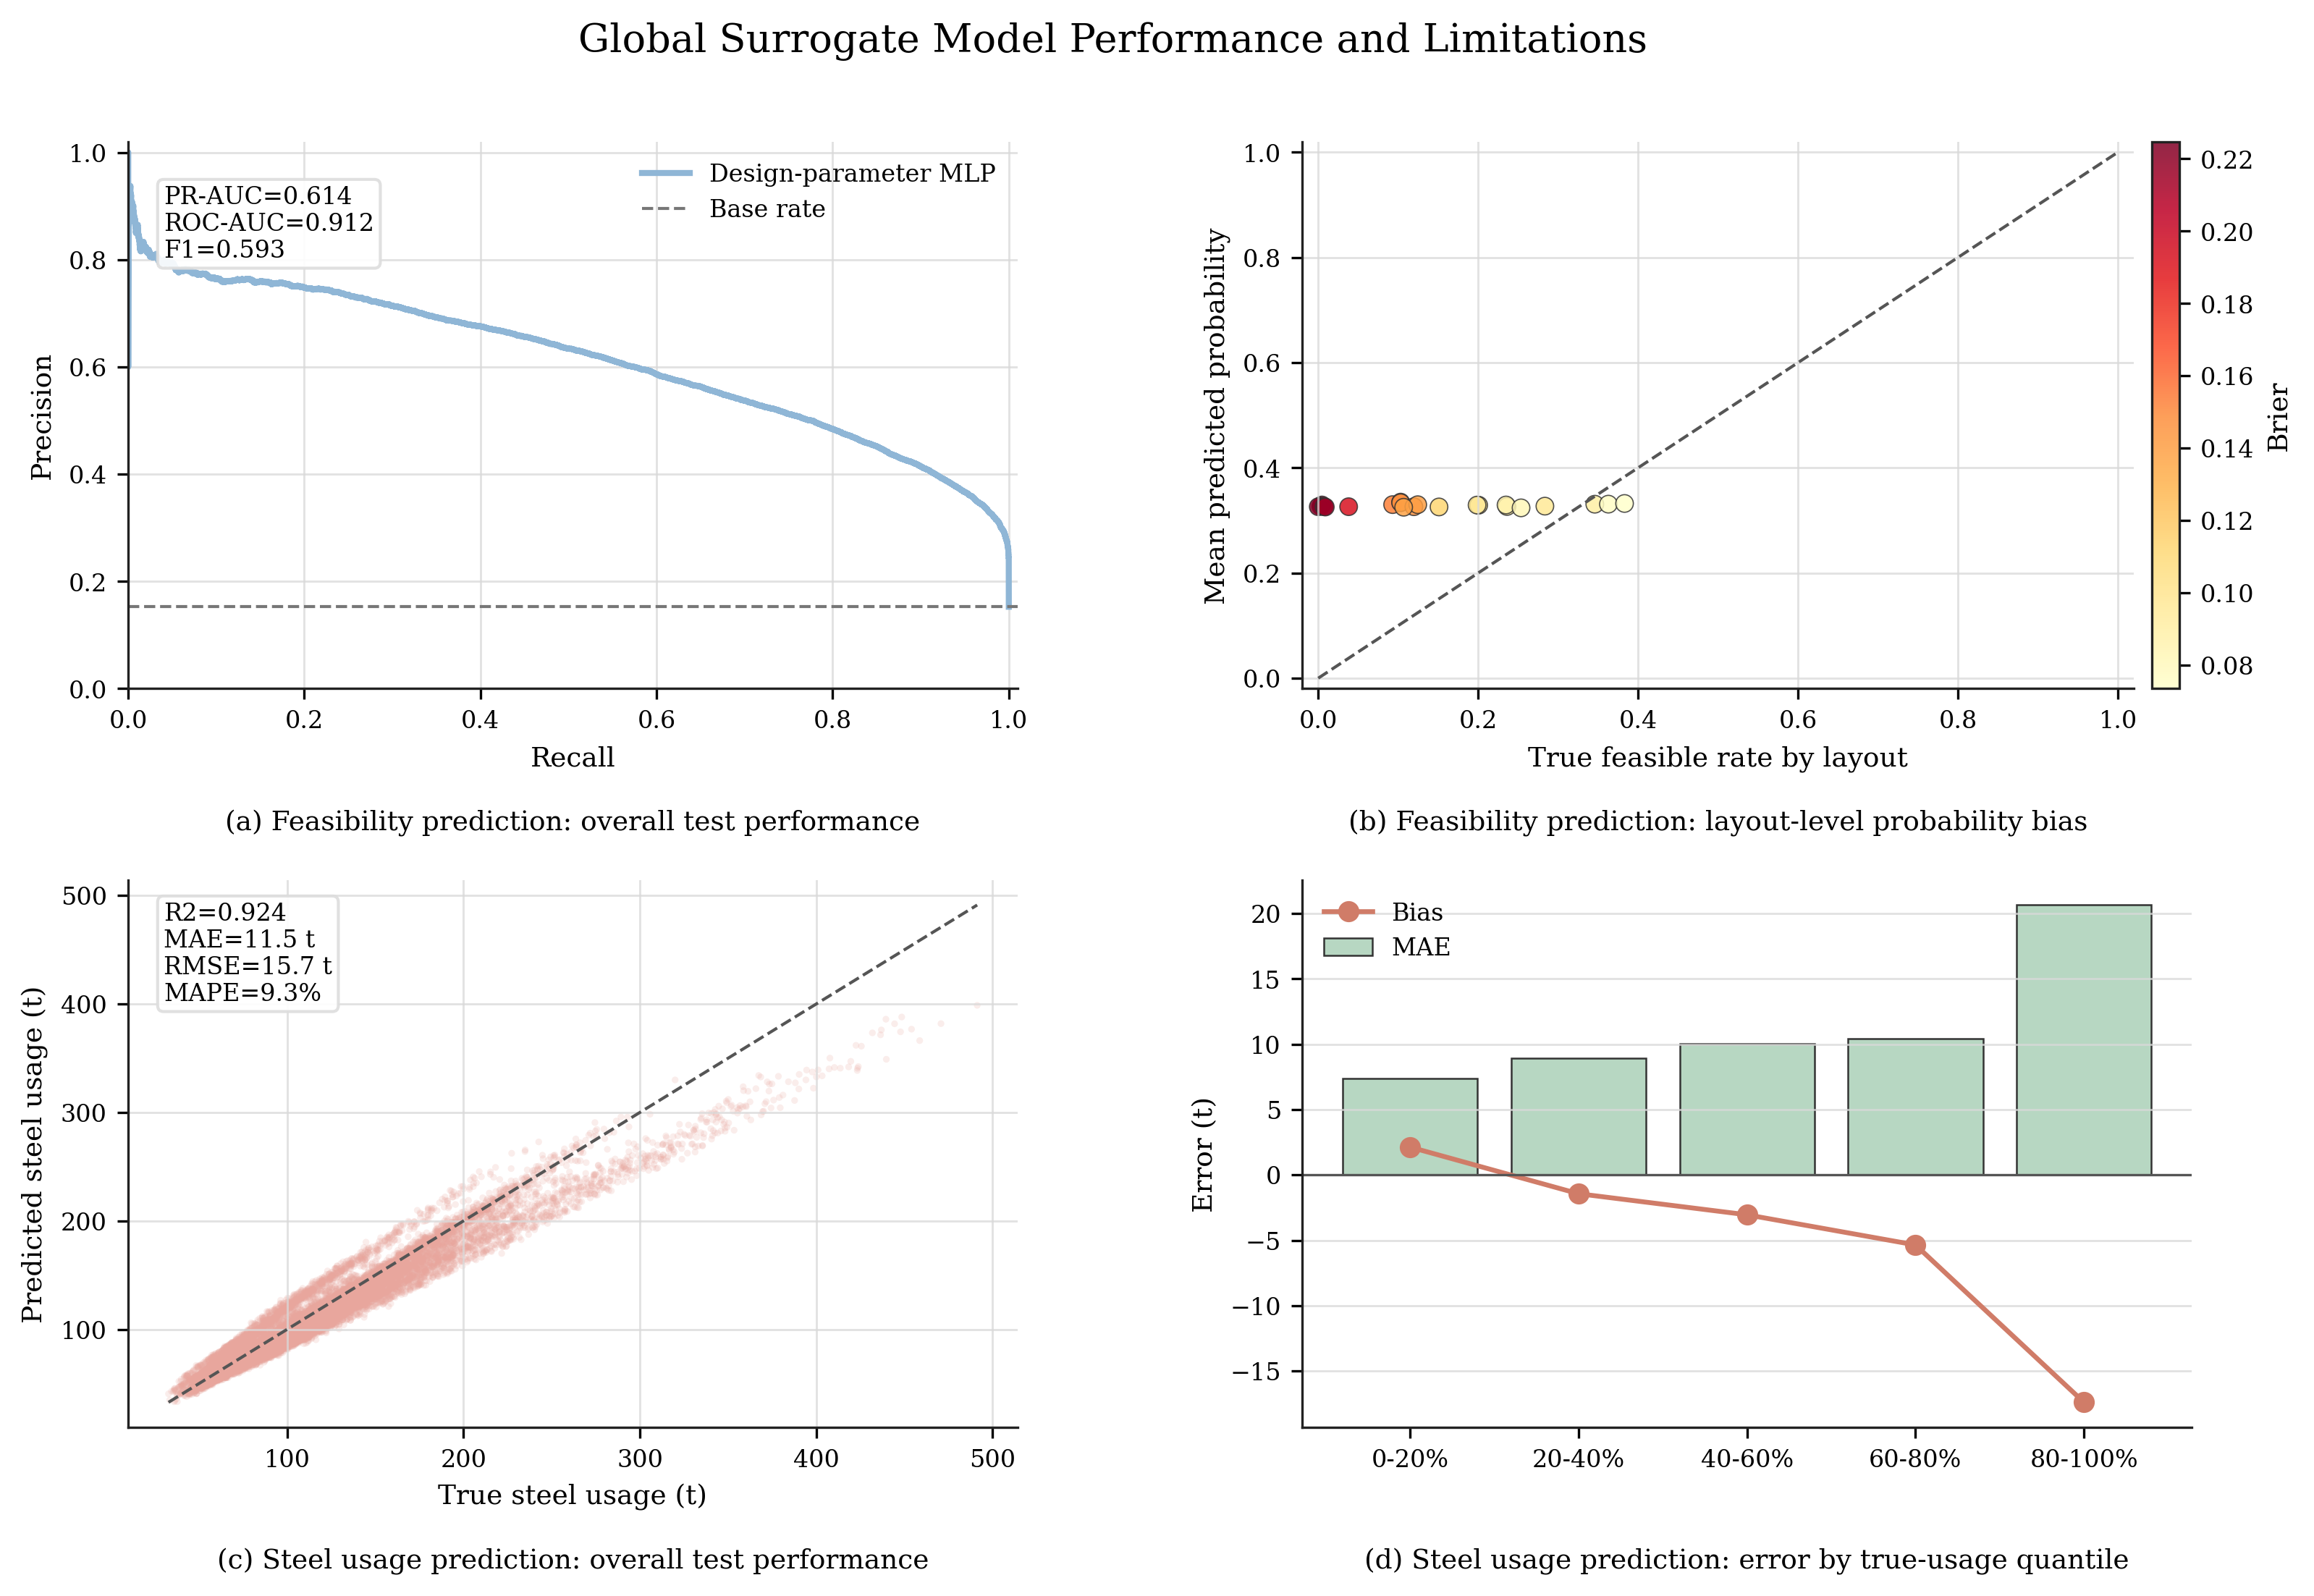
\includegraphics[width=\textwidth]{global_surrogate_overview.png}
\caption{Overall performance and error patterns of the global layout-conditioned surrogate model.}
\label{fig:global_surrogate_overview}
\end{figure*}


\begin{table*}[t]
\centering
\caption{Feasibility prediction performance of different surrogate input settings.}
\label{tab:global_feasibility_results}
\setlength{\tabcolsep}{5pt}
\begin{tabularx}{\textwidth}{@{}>{\raggedright\arraybackslash}X
>{\centering\arraybackslash}p{0.09\textwidth}
>{\centering\arraybackslash}p{0.09\textwidth}
>{\centering\arraybackslash}p{0.07\textwidth}
>{\centering\arraybackslash}p{0.105\textwidth}
>{\centering\arraybackslash}p{0.125\textwidth}
>{\centering\arraybackslash}p{0.145\textwidth}@{}}
\toprule
Model & ROC-AUC & PR-AUC & F1 & Reject rate & Feasible recall & False reject count \\
\midrule
Design-parameter MLP & 0.9117 & 0.6137 & 0.5927 & 0.4787 & 0.9946 & 90 \\
Layout-statistics MLP & 0.9547 & 0.8163 & 0.7370 & 0.4447 & 0.9994 & 10 \\
LayoutParamGNN & 0.9693 & 0.8593 & 0.7688 & 0.4736 & 0.9998 & 3 \\
\bottomrule
\end{tabularx}
\end{table*}


\begin{table*}[t]
\centering
\caption{Reinforcement usage prediction performance of different surrogate input settings.}
\label{tab:global_steel_results}
\setlength{\tabcolsep}{4pt}
\begin{tabularx}{\textwidth}{@{}>{\raggedright\arraybackslash}X
>{\centering\arraybackslash}p{0.075\textwidth}
>{\centering\arraybackslash}p{0.075\textwidth}
>{\centering\arraybackslash}p{0.06\textwidth}
>{\centering\arraybackslash}p{0.07\textwidth}
>{\centering\arraybackslash}p{0.075\textwidth}
>{\centering\arraybackslash}p{0.105\textwidth}
>{\centering\arraybackslash}p{0.09\textwidth}
>{\centering\arraybackslash}p{0.125\textwidth}@{}}
\toprule
Model & MAE (t) & RMSE (t) & $R^2$ & MAPE & Bias (t) & Pairwise acc. & Spearman & Top-10\% recall \\
\midrule
Design-parameter MLP & 32.30 & 45.77 & 0.351 & 0.247 & -13.89 & 0.9586 & 0.9547 & 0.8974 \\
Layout-statistics MLP & 13.83 & 18.75 & 0.891 & 0.112 & -1.66 & 0.9652 & 0.9628 & 0.9142 \\
LayoutParamGNN & 11.48 & 15.67 & 0.924 & 0.093 & -5.02 & 0.9787 & 0.9779 & 0.9483 \\
\bottomrule
\end{tabularx}
\end{table*}


\begin{figure*}[t]
\centering
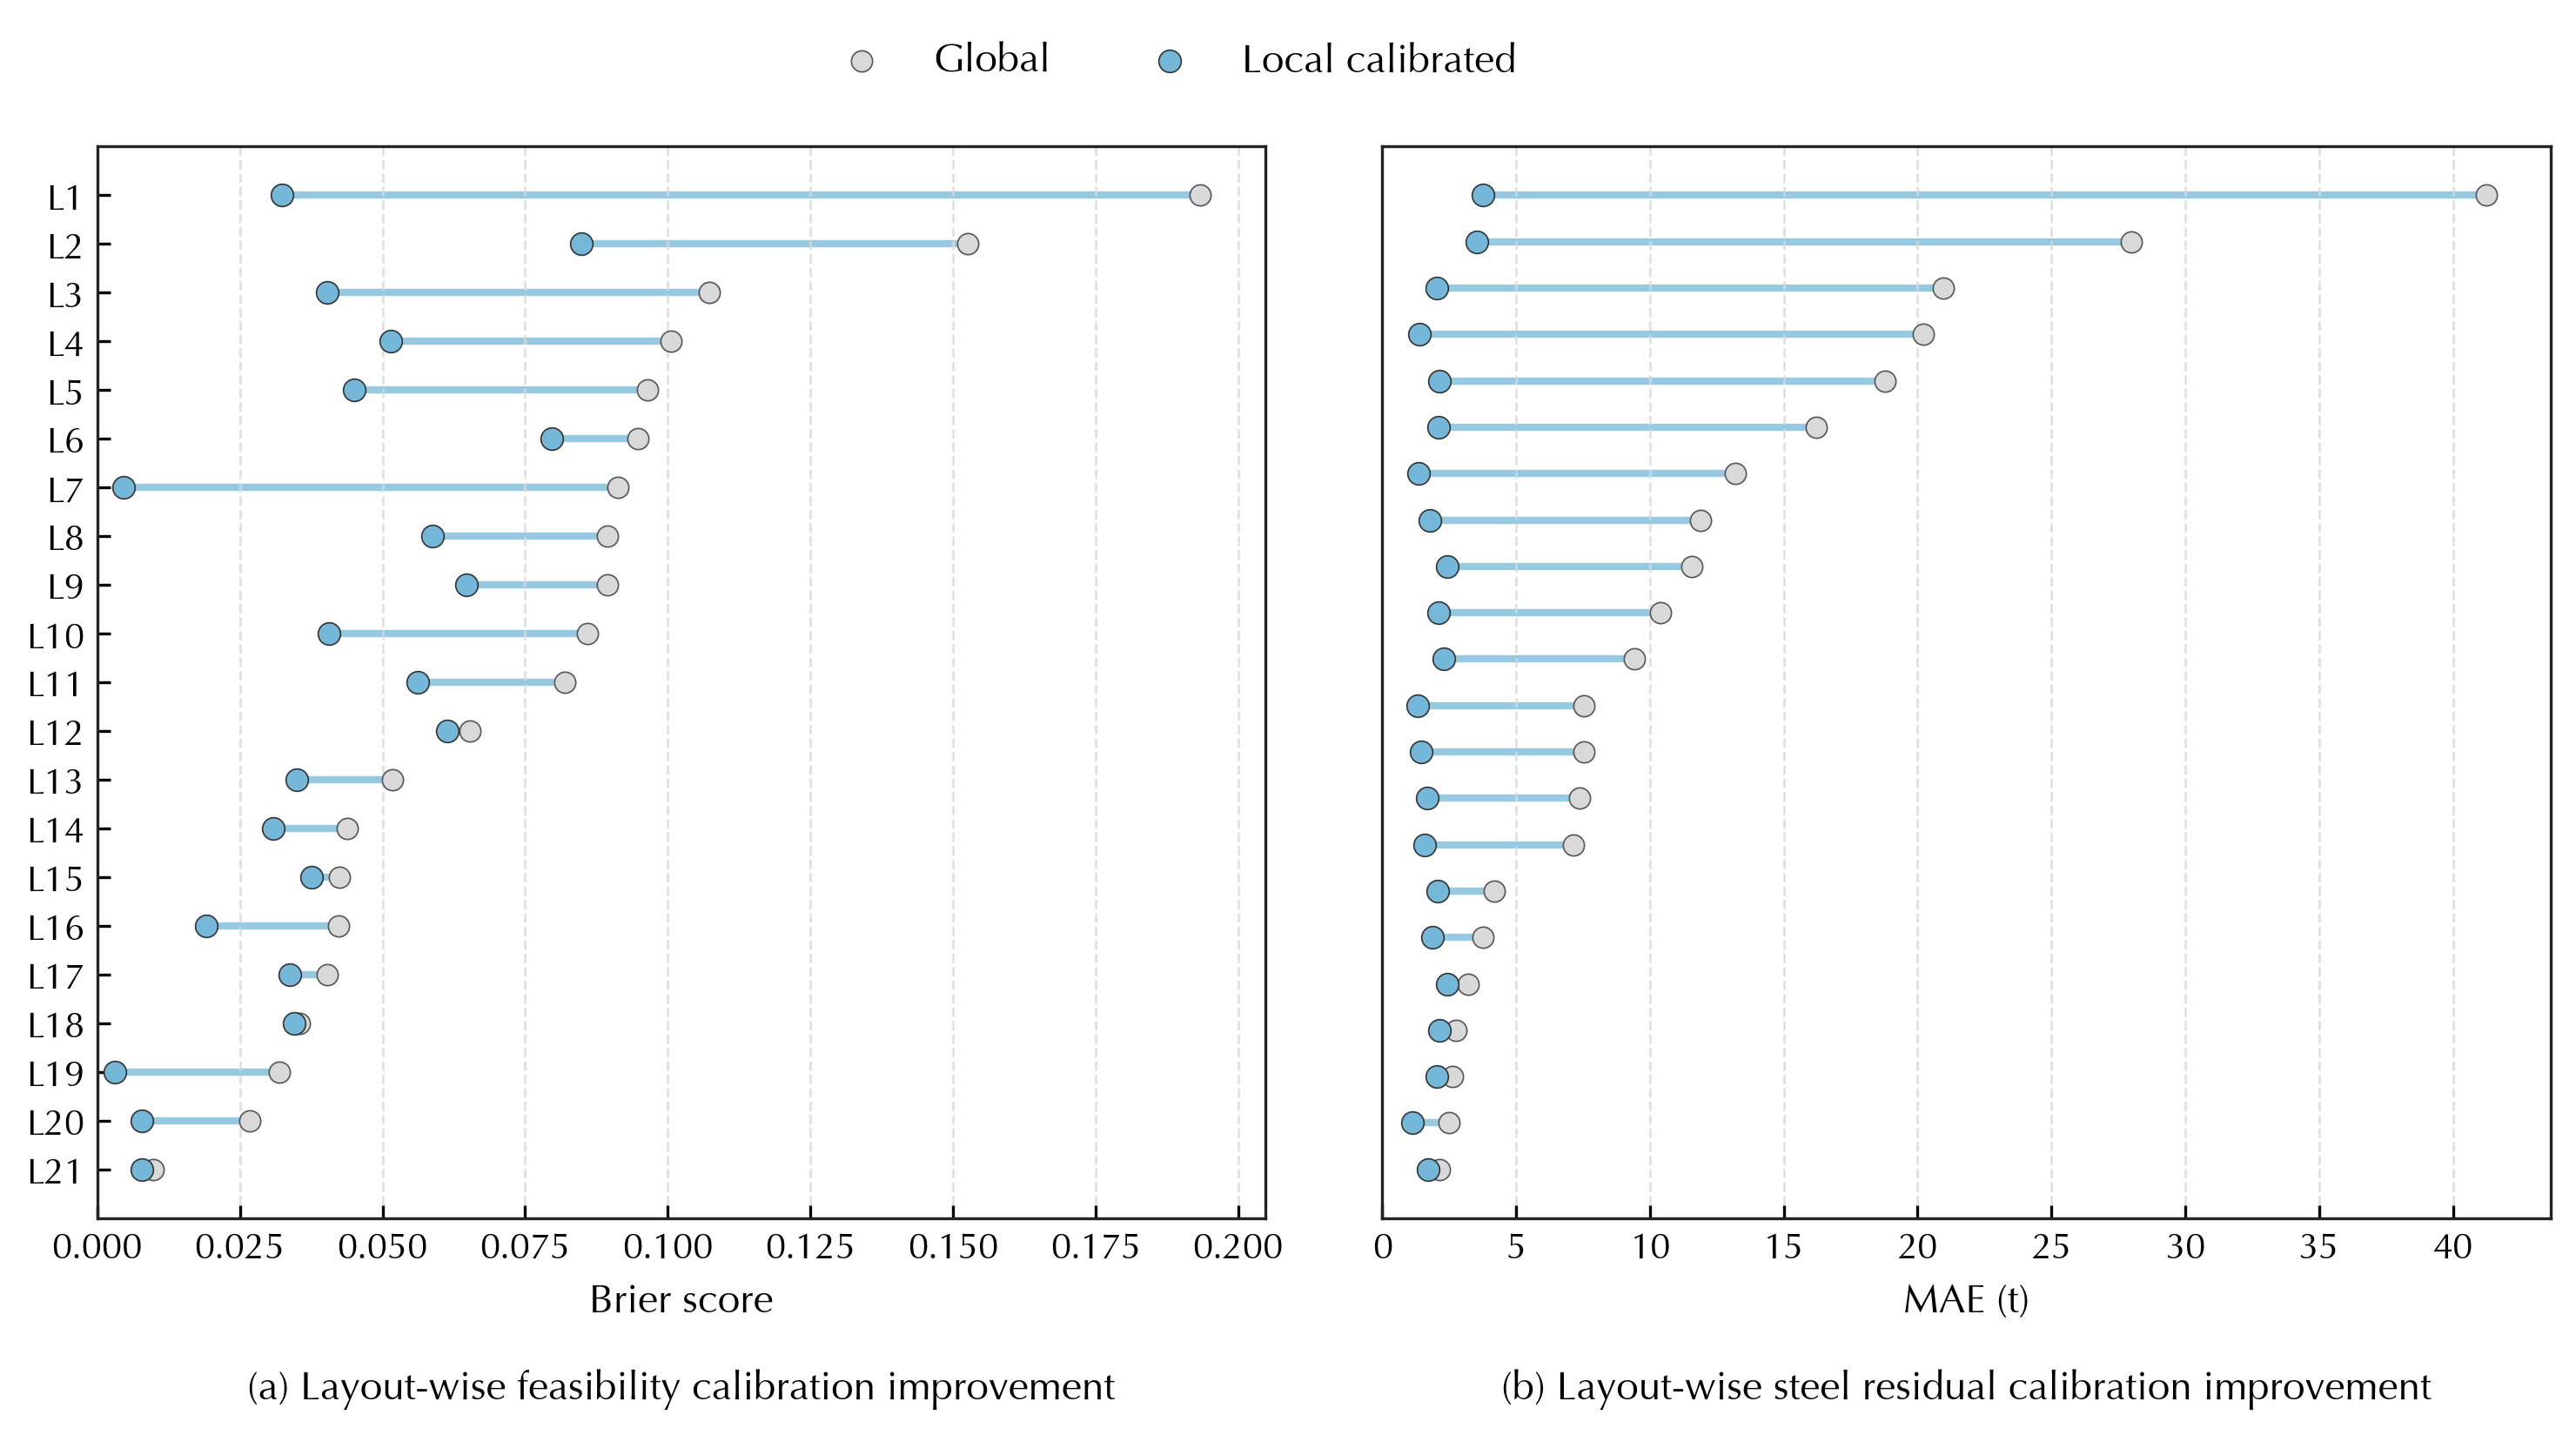
\includegraphics[width=\textwidth]{local_calibration_effect.png}
\caption{Effect of online local calibration using FEA-verified samples from the current layout.}
\label{fig:local_calibration_effect}
\end{figure*}


\begin{table}[t]
\centering
\caption{Representative local calibration results and local-only ablation using 100 FEA-verified samples.}
\label{tab:local_calibration_results}
\setlength{\tabcolsep}{2pt}
\begin{tabularx}{\columnwidth}{@{}>{\raggedright\arraybackslash}X>{\centering\arraybackslash}p{0.14\columnwidth}>{\centering\arraybackslash}p{0.17\columnwidth}>{\centering\arraybackslash}p{0.16\columnwidth}>{\centering\arraybackslash}p{0.13\columnwidth}@{}}
\toprule
Metric & Global & Local only & Calib. & Improv. \\
\midrule
\multicolumn{5}{@{}l}{\textit{Feasibility}} \\
Brier & 0.0749 & 0.0755 & 0.0437 & 42\% \\
ECE & 0.0895 & 0.0451 & 0.0333 & 63\% \\
Screen reject rate & 0.4708 & 0.5639 & 0.5481 & 16\% \\
Screen recall & 0.9990 & 0.7265 & 0.9939 & -1\% \\
\midrule
\multicolumn{5}{@{}l}{\textit{Steel}} \\
MAE & 11.48~t & 4.82~t & 2.04~t & 82\% \\
RMSE & 12.30~t & 5.64~t & 2.76~t & 78\% \\
$R^2$ & 0.847 & 0.976 & 0.994 & 17\% \\
MAPE & 9.26\% & 3.26\% & 1.64\% & 82\% \\
\bottomrule
\end{tabularx}
\end{table}


\begin{figure*}[t]
\centering
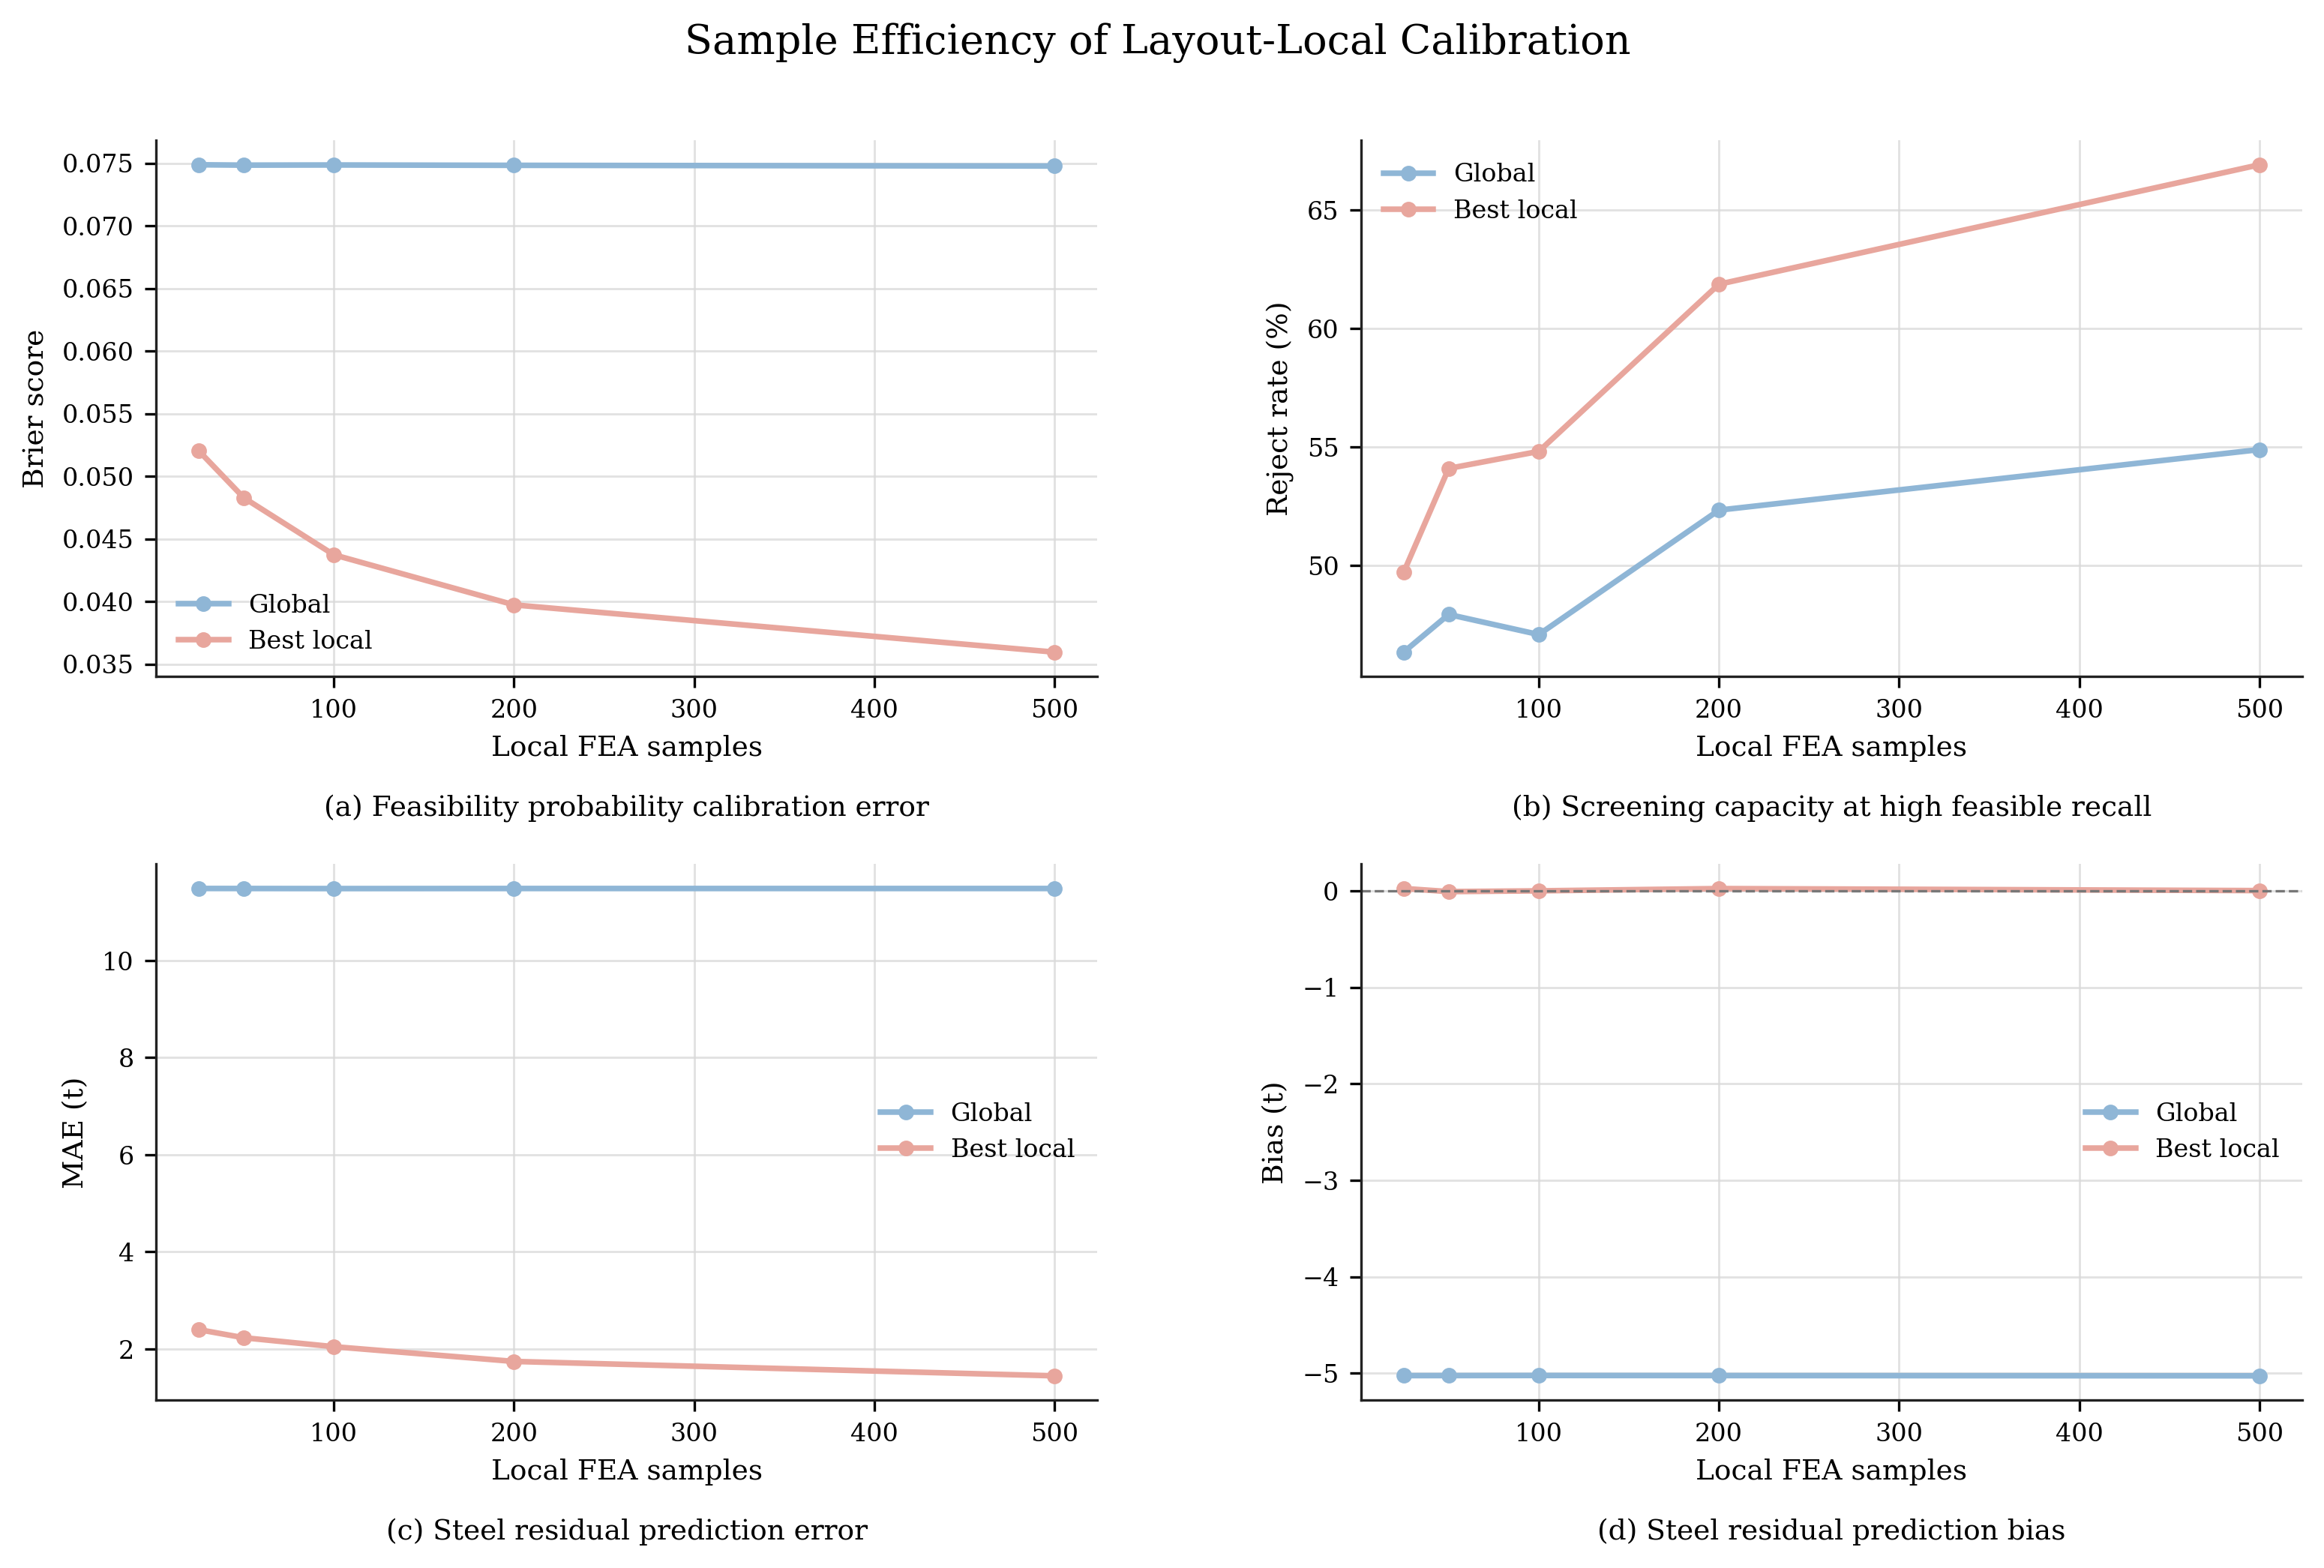
\includegraphics[width=\textwidth]{calibration_sample_efficiency.png}
\caption{Sample efficiency of online local calibration under different numbers of local FEA-verified samples.}
\label{fig:calibration_sample_efficiency}
\end{figure*}

\subsection{Dataset and Structural Evaluation}
\label{subsec:dataset_structural_evaluation}

The dataset is constructed from engineering shear wall layouts and a parametric structural evaluation workflow. Each sample corresponds to a layout, a design condition, and a section-material design scheme. The input includes layout information and design parameters, and the supervised labels include the comprehensive feasibility label $y_f$ and the reinforcement usage $m_s$.

The dataset contains 143 shear wall layouts designed by professional engineers, which can be divided into three groups according to seismic intensity and building height. Group7-H1 corresponds to low-demand cases with seismic intensity 7, PGA of 0.10~g, and building height $H \leq 50$~m. Group7-H2 corresponds to medium-demand cases with the same seismic intensity but building height $H>50$~m. Group8 corresponds to high-demand cases with seismic intensity 8 and PGA of 0.20~g. These groups reflect the combined influence of seismic demand and structural height on shear wall section design and material usage.

For each layout, 5000 candidate design schemes are sampled from a predefined parameter space, which is summarized in Table~\ref{tab:parameter_space}. The sampled variables include the number of stories, wall thicknesses in different vertical zones, main and secondary beam dimensions, concrete strength grade, seismic intensity, site class, and seismic group. During sampling, wall thicknesses are constrained to be nonincreasing along the building height, i.e., $t_{w,t}\le t_{w,m}\le t_{w,b}$.

Representative finite element models generated from the same parametric workflow are shown in Fig.~\ref{fig:model_cases}.


A true structural evaluator $\mathcal{E}$ is used to generate labels for all sampled candidates. For each candidate, the evaluator automatically constructs the structural model, performs FEA in OpenSees\cite{McKenna2011OpenSees}, extracts global structural responses and member forces, and conducts code-based member design and reinforcement calculation. The comprehensive feasibility label $y_f$ is determined by analysis validity, global response limits, and member-level design checks. The reinforcement usage label $m_s$ is obtained from the final member design results.

The resulting dataset contains 715,000 FEA-labeled samples. After removing cases with failed analyses or invalid results, the final dataset contains 714,972 samples. A layout-level split is adopted to evaluate cross-layout generalization. Specifically, 100 layouts are used for training, 21 layouts for validation, and 22 layouts for testing, corresponding to an approximate ratio of 0.70:0.15:0.15. All parameter variants of the same layout are assigned to the same subset to avoid information leakage between training and testing. The test layouts cover the three design-condition groups and are used for global surrogate evaluation, local calibration analysis, and optimization benchmarking.

 The detailed distribution of layouts and samples across design-condition groups is given in Table~\ref{tab:dataset_split}.


\subsection{Global Surrogate Model Training}
\label{subsec:global_surrogate_training}

Two global surrogate models are trained, i.e. the feasibility surrogate $SM_f$ and the reinforcement usage surrogate $SM_s$. They use the same candidate representation and model architecture, but are trained separately with independent parameters for different prediction tasks. The feasibility surrogate outputs the probability that a candidate can pass the comprehensive structural checks, while the reinforcement surrogate predicts the reinforcement quantity before true evaluation.

To examine the effect of layout representation, three model settings are compared. The Design-parameter MLP uses only section, material, and design-condition parameters, the Layout-statistics MLP further incorporates global layout statistics, and the LayoutParamGNN jointly uses the room-level graph, global layout statistics, and design parameters. Here, global layout statistics refer to fixed-dimensional tabular descriptors computed from the overall shear wall layout, such as plan aspect ratio, shear wall ratio, total wall length, centroid-related measures, and other geometric summaries, which convert layouts with variable numbers of wall components into fixed-length features.

The LayoutParamGNN adopts a three-layer GraphSAGE encoder for room-graph feature extraction\cite{Hamilton2017GraphSAGE}. In each surrogate model, the graph-level representation is fused with global layout statistics and design-parameter embeddings before being passed to the task-specific output layer. For the feasibility model, the hidden dimension, dropout rate, batch size, and learning rate are set to 256, 0.2, 128, and 0.001, respectively. Weighted binary cross-entropy is used to handle class imbalance. The screening threshold is selected on the validation set according to a target feasible recall of 0.995, and the default classification threshold of 0.5 is not used.

For the reinforcement model, the hidden dimension, dropout rate, batch size, and learning rate are set to 128, 0.1, 512, and 0.0005, respectively. Both global surrogate models are trained using validation-based early stopping.


\subsection{Local Calibration Settings}
\label{subsec:local_calibration_settings}

Local calibration experiments are conducted on the test layouts to simulate the use of FEA-verified samples accumulated during optimization. For each test layout, a certain number of verified samples are randomly selected as the local calibration set, and the remaining samples are used as the layout-specific evaluation set. Each local calibration sample stores the candidate representation, the global surrogate predictions, and the true FEA-based labels.

The calibration objects are the feasibility probability and the reinforcement residual. For feasibility calibration, the global feasibility probability is first transformed into the logit space and then combined with the design parameters as the calibration input, while the target is the true feasibility label. Several lightweight calibration methods are compared, including Platt scaling\cite{Platt1999} and isotonic regression\cite{Zadrozny2002}. In addition, residual-based probability correction and ensemble voting/averaging are tested as simple empirical alternatives for local probability adjustment \cite{Bella2013}. The calibrated probabilities are used to assess probability reliability and conservative screening performance.

For reinforcement calibration, the model learns the residual between the true reinforcement usage and the global surrogate prediction. The input consists of the global reinforcement prediction and design parameters, while the target is the reinforcement residual. Ridge regression\cite{Hoerl1970Ridge}, Gaussian process regression\cite{Rasmussen2006GPML}, LightGBM\cite{Ke2017LightGBM}, and K-nearest neighbors\cite{Cover1967KNN} are compared as lightweight residual calibration models. These comparisons test whether the systematic error of the global model can be corrected with a small number of layout-specific FEA samples.

To examine sample efficiency, local calibration sizes of 25, 50, 100, 200, and 500 samples are considered. Each setting is repeated three times with different random samples, and the average results are reported. In the online optimization experiments, local calibration is activated only after at least 25 FEA-verified samples have been accumulated for the current layout. The feasibility screening threshold follows the same conservative principle as the global model, with a target feasible recall of 0.995 and a threshold scale factor of 0.1. When the local samples are insufficient or contain only one class for the feasibility task, the framework falls back to the global surrogate prediction and the validation-based global threshold.

\subsection{Optimization Benchmark Settings}
\label{subsec:optimization_benchmark_settings}

Optimization experiments are conducted on 15 unseen layouts selected from the test set, with five layouts from each design-condition group. For each layout, five random seeds are used. For each test layout, the layout $L$ and design condition $c$ are fixed, and the optimization variables are the section and material parameters $x$. All compared methods use the same design space, true evaluator, and random seeds.

Genetic algorithm is adopted as the main optimizer\cite{Goldberg1989}. In the experiments, the population size, number of generations, mutation rate, and elite size are set to 48, 15, 0.30, and 2, respectively. To examine whether the surrogate-assisted mechanism depends on a specific optimizer, particle swarm optimization (PSO) and random search are also included as supplementary optimizers\cite{Kennedy1995PSO}. The PSO uses a swarm size of 48 and 15 iterations, with a mutation rate of 0.15 to improve exploration. The random search baseline evaluates 720 candidates in batches of 48.

Three candidate evaluation strategies are compared:
\begin{enumerate}
\item \textbf{Full FEA optimization}: all candidates generated by the optimizer are evaluated by $\mathcal{E}$. This strategy serves as the baseline.
\item \textbf{Cost ranking}: candidates are ranked using the reinforcement surrogate and the estimated concrete quantity, and only high-priority candidates are submitted to $\mathcal{E}$.
\item \textbf{Screen \& cost ranking}: feasibility screening, reinforcement-based cost ranking, and online local calibration are jointly used to select candidates for true FEA evaluation.
\end{enumerate}

For surrogate-assisted strategies, each optimizer first generates a candidate batch $\mathcal{B}_t$. The surrogate module then evaluates all candidates in the batch and selects a subset $\mathcal{S}_t$ for true FEA and code checking. A minimum number of evaluated candidates is enforced to avoid overly aggressive filtering. In the experiments, the minimum number of true evaluations per batch is set to \texttt{min\_eval} = 8. The verified results are used to update the optimizer and the local calibration set. Candidates not selected for FEA are not used as true samples and are not considered in final best-solution comparison.

The cost-ranking uses an evaluation ratio of 0.8 before the first feasible design is found and 0.5 afterwards. After a feasible design has been observed, the selected subset is allocated to cost ranking, feasibility-risk ranking, and random exploration with ratios of 0.60, 0.25, and 0.15, respectively. The feasibility-risk term in the surrogate ranking score uses a hinge target of $p_0=0.5$ and a penalty coefficient of $\eta=1.0\times10^6$. Candidates rejected by surrogate screening or skipped after cost ranking are assigned $M_{rej}=1.0\times10^{12}$. For FEA-evaluated infeasible candidates, the scalar penalty uses $P_0=1.0\times10^5$, $\lambda_v=1.0\times10^7$, and $\lambda_c=0.01$.

\subsection{Evaluation Metrics}
\label{subsec:evaluation_metrics}

Definitions of the full set of metrics used in this study are provided in \ref{app:evaluation_metrics}.

The feasibility surrogate is assessed using ROC-AUC, PR-AUC, and F1 score to characterize overall classification performance. Because it is used as a conservative screening tool, feasible recall, reject rate, and false reject count are also reported to quantify the retained feasible candidates, the candidates filtered before FEA, and the feasible candidates mistakenly rejected by the screen.

Reinforcement prediction accuracy is measured by mean absolute error (MAE), root mean square error (RMSE), coefficient of determination ($R^2$), mean absolute percentage error (MAPE), and bias. To reflect its role in candidate ranking, pairwise ranking accuracy, Spearman correlation, and top-$k$ recall are further included.

Local calibration is evaluated from both probability and residual-correction perspectives. Feasibility probability calibration is measured by Brier score\cite{Brier1950} and expected calibration error (ECE)\cite{Naeini2015}, together with screening recall and reject rate, whereas reinforcement residual calibration is measured by MAE, RMSE, bias, and the ranking metrics after calibration.

Optimization performance is summarized in terms of computational efficiency and solution quality. Efficiency is measured by the number of true FEA calls and the FEA reduction ratio, while solution quality is characterized by feasible-solution discovery rate, the number of FEA calls required to find the first feasible solution, and final material cost. For each test layout and random seed, surrogate-assisted strategies are compared with full FEA optimization to determine whether FEA calls can be reduced without substantial degradation in feasibility discovery or final cost.
 % experiments

\section{Experimental Results and Discussions}
\label{sec:results_discussion}

\subsection{Global Surrogate Model Performance}
\label{subsec:global_surrogate_results}

Tables~\ref{tab:global_feasibility_results} and~\ref{tab:global_steel_results} compare the three surrogate models under progressively enriched input settings. For feasibility prediction, the Param-MLP achieves a PR-AUC of 0.6137 and an F1 score of 0.5927 on unseen layouts. Incorporating global layout statistics substantially improves these values to 0.8163 and 0.7370, corresponding to relative improvements of 33.0\% and 24.3\%, respectively. This result indicates that layout-level geometric information is essential for cross-layout prediction. The proposed FuseGNN further increases the PR-AUC to 0.8593 and the F1 score to 0.7688, indicating that the room-level graph captures spatial and topological information that cannot be fully represented by manually defined global statistics.

More importantly, the FuseGNN provides a favorable balance between candidate rejection and feasible-solution retention. Under the selected screening threshold, it rejects approximately 47.36\% of the candidates while maintaining a feasibility recall of 0.9998, with only three feasible samples falsely rejected. This conservative screening performance is substantially better than that of the parameter-only model and also improves upon the statistics-based model, supporting its use for removing low-feasibility candidates before FEA.

A similar pattern is observed for reinforcement prediction. The Param-MLP produces an MAE of 32.30~t and an $R^2$ of 0.351, confirming that design parameters alone are insufficient to represent layout-dependent reinforcement demand. Adding global layout statistics reduces the MAE to 13.83~t, while the FuseGNN further lowers it to 11.48~t and increases the $R^2$ to 0.924. It also achieves high pairwise ranking accuracy, Spearman correlation, and top-10\% recall. Since the reinforcement surrogate is primarily used for candidate ranking rather than exact quantity estimation, these results demonstrate that the proposed representation can reliably identify candidates with relatively low reinforcement demand within each layout.

Fig.~\ref{fig:global_surrogate_overview} further illustrates the prediction behavior of the FuseGNN. The precision-recall curve in Fig.~\ref{fig:global_surrogate_overview}(a) shows that the graph-based feasibility model achieves a much better precision-recall trade-off than the baseline feasible rate. However, the layout-wise probability comparison in Fig.~\ref{fig:global_surrogate_overview}(b) reveals that prediction bias still exists for some layouts. Several layouts with low true feasible rates are assigned overly optimistic feasibility probabilities. The reinforcement error distribution in Fig.~\ref{fig:global_surrogate_overview}(d) also shows that the prediction error becomes more biased in high-reinforcement regions. In the highest 20\% reinforcement-usage interval, the MAE increases to approximately 20.7~t and the bias reaches about $-17.4$~t. Therefore, although the FuseGNN model provides effective feasibility screening and reinforcement ranking, its layout and demand dependent errors make it insufficient for direct optimization without further calibration.


\begin{table}[!t]
\centering
\setcounter{table}{4}
\caption{Representative local calibration results and local-only ablation using 100 FEA-verified samples.}
\label{tab:local_calibration_results}
\setlength{\tabcolsep}{2pt}
\begin{threeparttable}
\begin{tabularx}{\columnwidth}{@{}>{\raggedright\arraybackslash}X>{\centering\arraybackslash}p{0.14\columnwidth}>{\centering\arraybackslash}p{0.17\columnwidth}>{\centering\arraybackslash}p{0.16\columnwidth}>{\centering\arraybackslash}p{0.13\columnwidth}@{}}
\toprule
Metric & Global & Local only & Calib. & Improv. \\
\midrule
\multicolumn{5}{@{}l}{\textit{Feasibility}} \\
Brier & 0.0749 & 0.0755 & 0.0437 & 42\% \\
ECE & 0.0895 & 0.0451 & 0.0333 & 63\% \\
feasibility recall & 0.9990 & 0.7265 & 0.9939 & -1\% \\
reject rate & 0.4708 & 0.5639 & 0.5481 & 16\% \\
\midrule
\multicolumn{5}{@{}l}{\textit{Steel}} \\
MAE & 11.48~t & 4.82~t & 2.04~t & 82\% \\
RMSE & 12.30~t & 5.64~t & 2.76~t & 78\% \\
$R^2$ & 0.847 & 0.976 & 0.994 & 17\% \\
MAPE & 9.26\% & 3.26\% & 1.64\% & 82\% \\
\bottomrule
\end{tabularx}

\begin{tablenotes}[flushleft]
\footnotesize
\item \textit{Note:} Global: uncalibrated global surrogate; Local only: model trained directly on current-layout samples without global predictions; Calib.: proposed local calibration of the global surrogate; Improv.: relative change from Global to Calib.
\end{tablenotes}

\end{threeparttable}
\end{table}
% \setcounter{table}{6}


\begin{table*}[!t]
\centering
\setcounter{table}{5}
\caption{Optimization efficiency and solution quality under different candidate evaluation strategies.}
\label{tab:optimization_summary_results}
\small
\setlength{\tabcolsep}{3.5pt}
\begin{tabularx}{\textwidth}{@{}>{\raggedright\arraybackslash}p{0.13\textwidth}
>{\raggedright\arraybackslash}p{0.13\textwidth}
>{\centering\arraybackslash}p{0.055\textwidth}
>{\centering\arraybackslash}p{0.095\textwidth}
>{\centering\arraybackslash}X
>{\centering\arraybackslash}p{0.105\textwidth}
>{\centering\arraybackslash}X
>{\centering\arraybackslash}p{0.12\textwidth}@{}}
\toprule
Algorithm & Method & Runs & Success rate & Mean FEA calls & FEA reduction & First feasible FEA & Cost ratio vs. full \\
\midrule
\multirow{3}{*}{GA}
& Full FEA & 75 & 68.0\% & 650 & -- & 72 & -- \\
& Cost ranking & 75 & 60.0\% & 279 & 57.0\% & 24 & 1.016 \\
& Screen \& ranking & 75 & 65.3\% & 223 & 65.7\% & 28 & 1.018 \\
\midrule
\multirow{3}{*}{PSO}
& Full FEA & 75 & 61.3\% & 573 & -- & 105 & -- \\
& Cost ranking & 75 & 57.3\% & 261 & 54.4\% & 56 & 1.006 \\
& Screen \& ranking & 75 & 58.7\% & 215 & 62.4\% & 51 & 1.017 \\
\midrule
\multirow{3}{*}{Random search}
& Full FEA & 75 & 68.0\% & 717 & -- & 71 & -- \\
& Cost ranking & 75 & 66.7\% & 358 & 50.1\% & 42 & 1.000 \\
& Screen \& ranking & 75 & 66.7\% & 247 & 65.6\% & 31 & 1.002 \\
\bottomrule
\end{tabularx}

\vspace{0.8em}

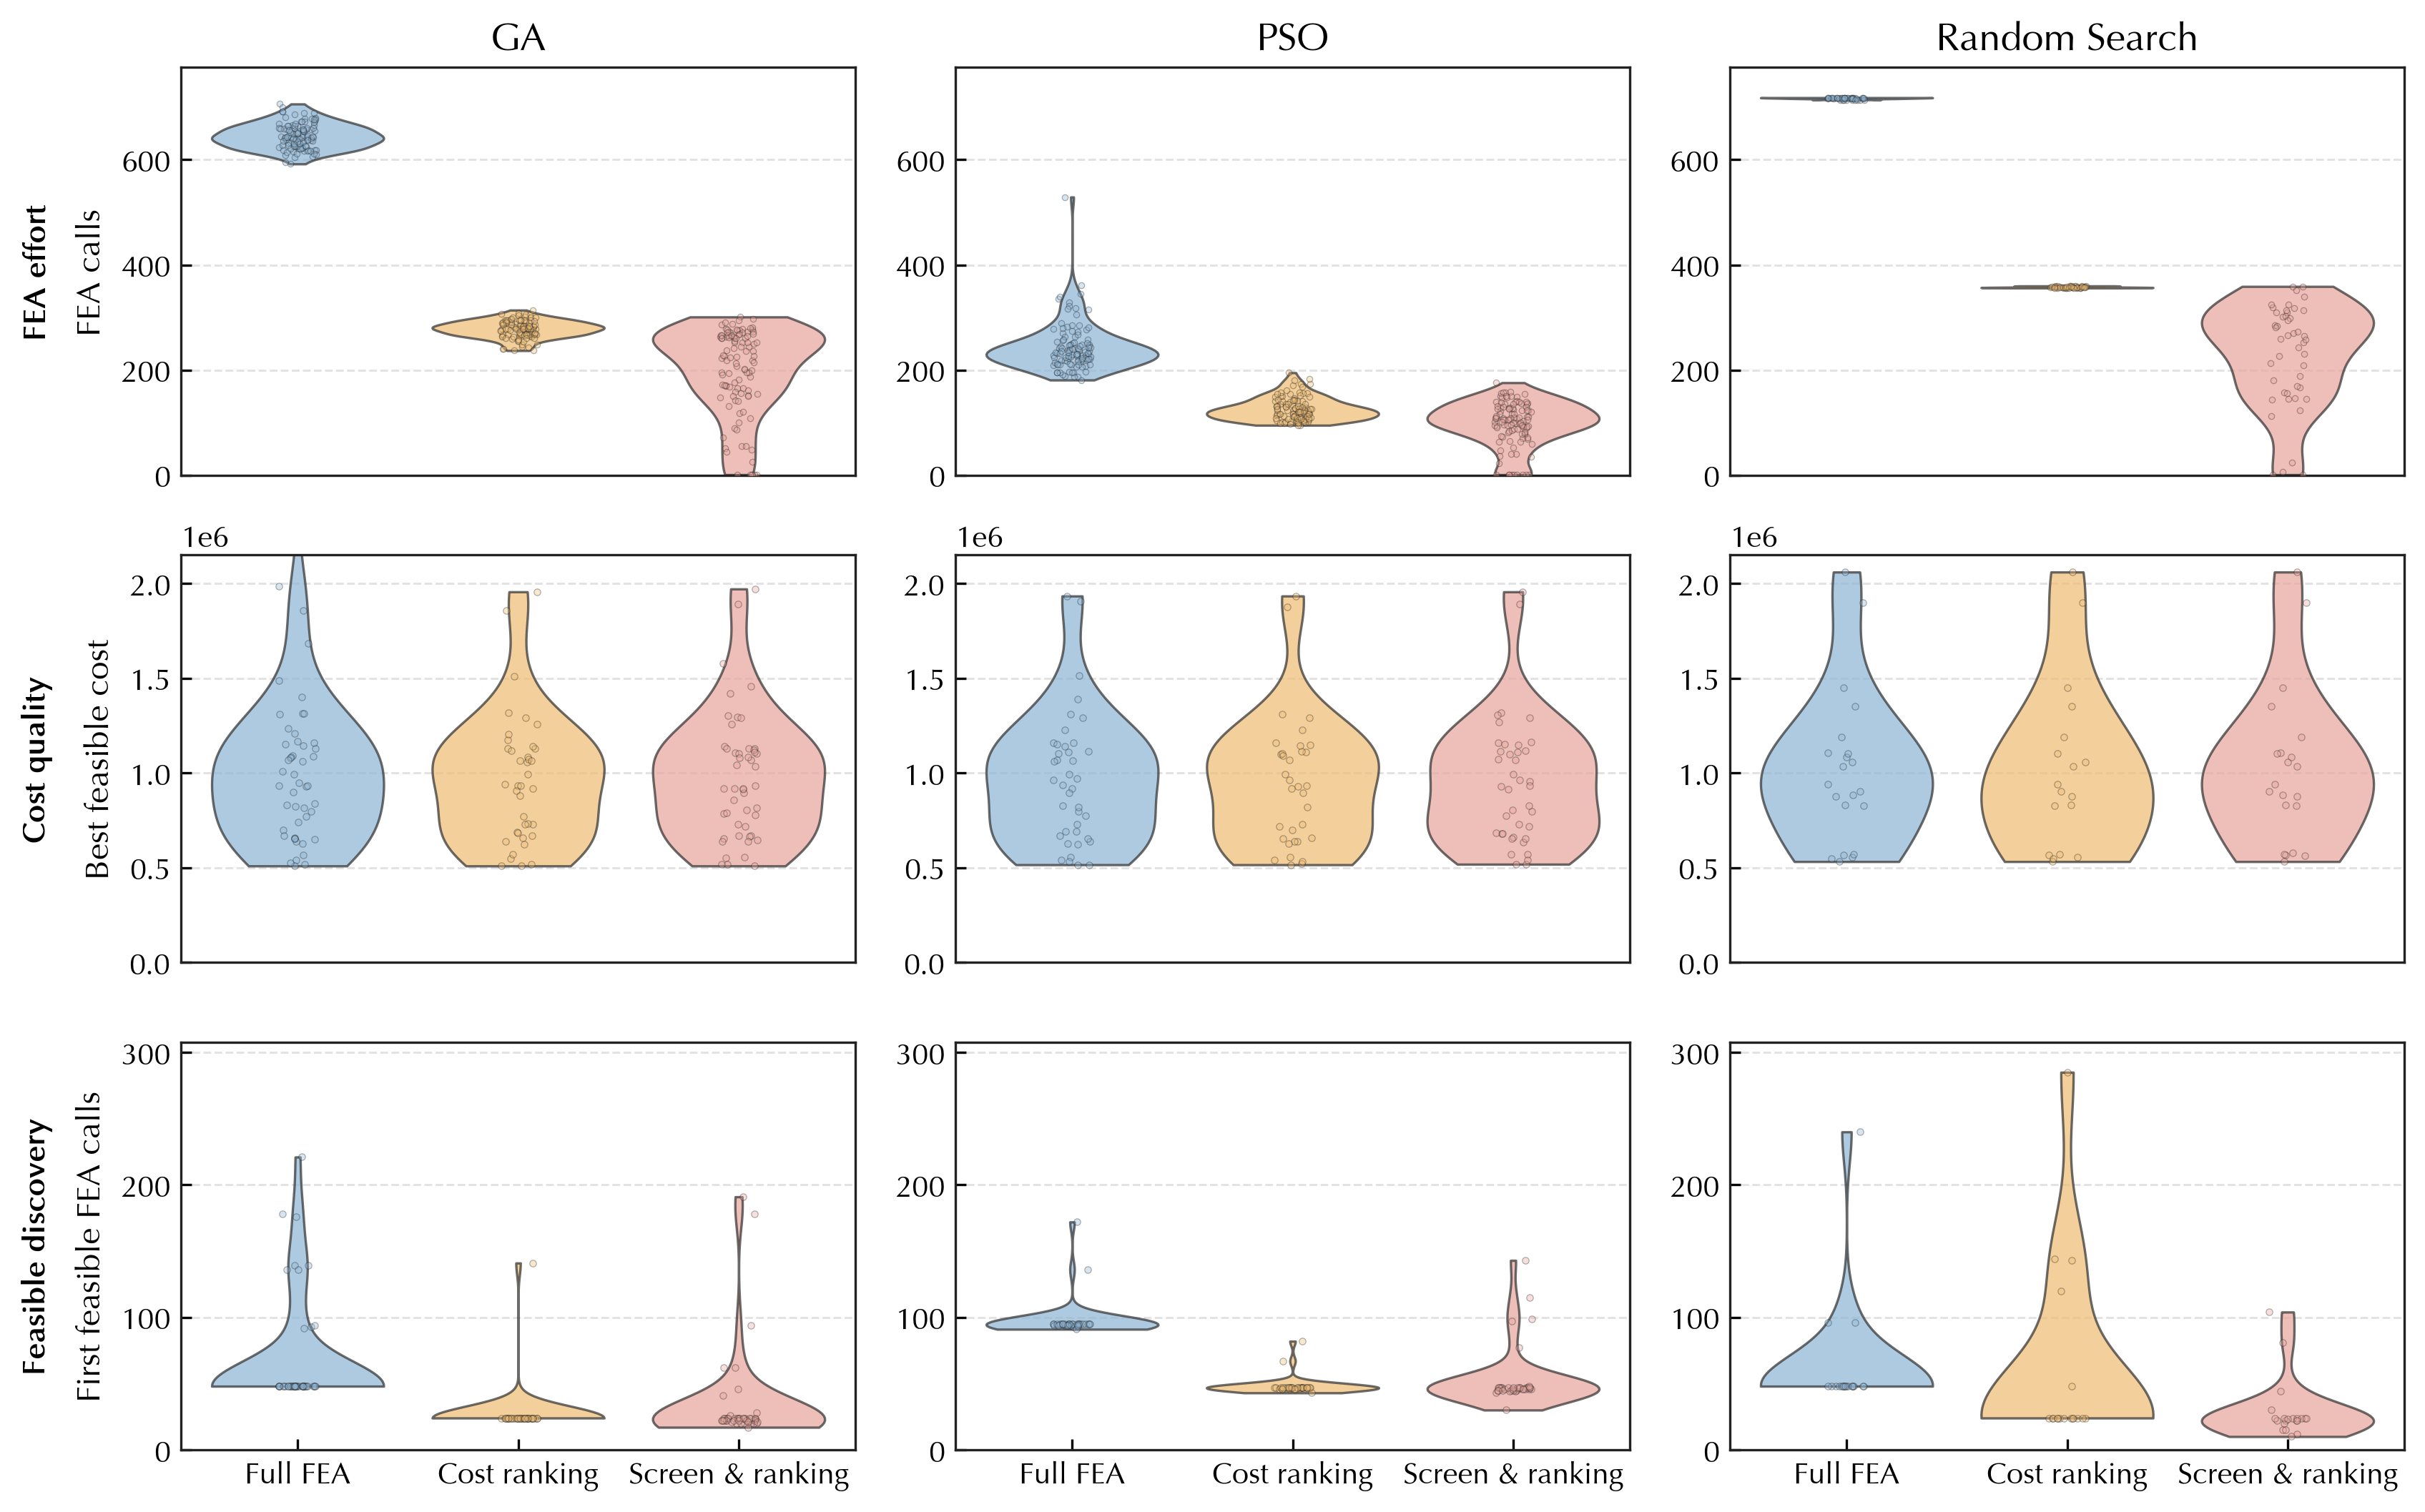
\includegraphics[width=\textwidth]{optimization_benchmark_results.pdf}
\captionsetup{labelfont=normalfont,textfont=normalfont,labelsep=colon,justification=centering,singlelinecheck=true}
\captionof{figure}{Optimization efficiency and solution quality under different optimizers and candidate evaluation strategies.}
\label{fig:optimization_benchmark_results}
\end{table*}

\begin{figure*}[t]
\centering
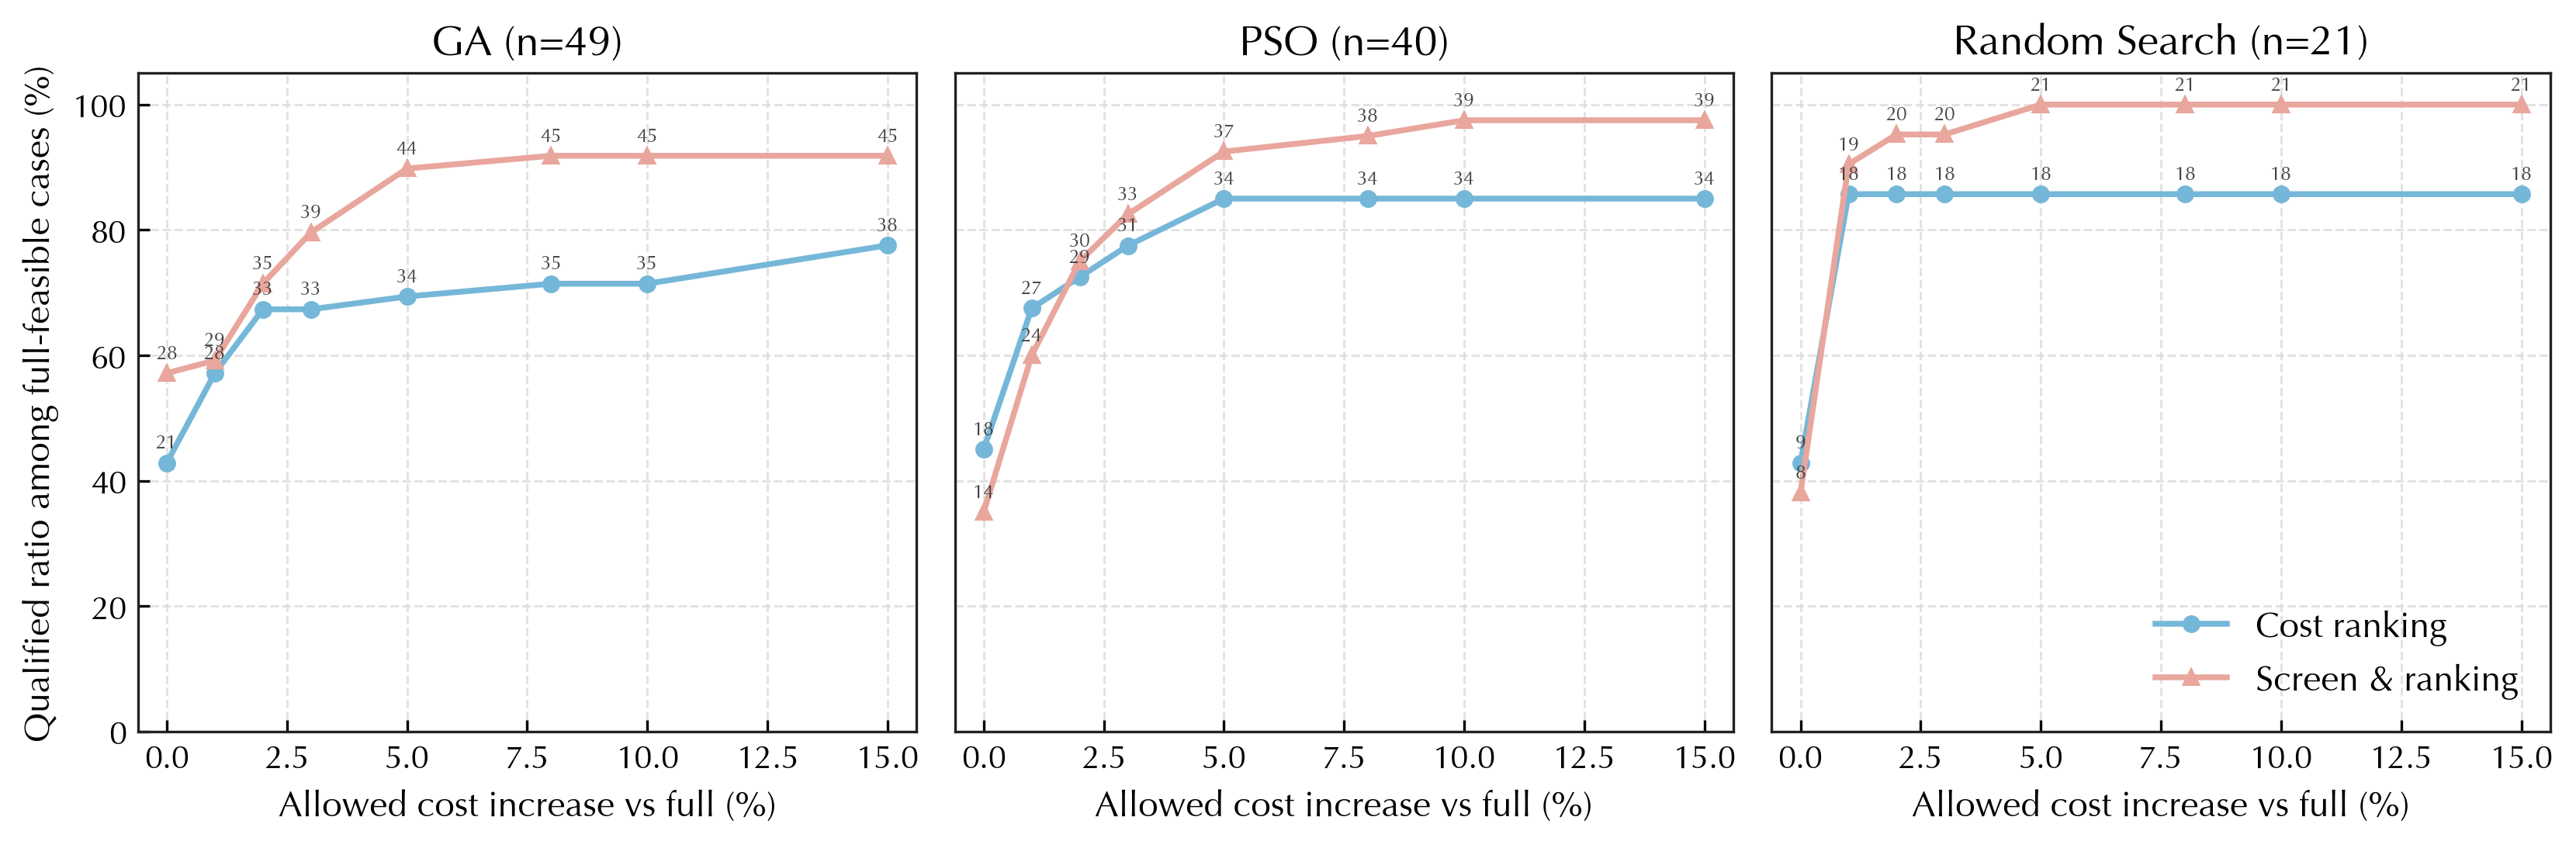
\includegraphics[width=\textwidth]{cost_tolerance_analysis.pdf}
\caption{Cost-tolerance analysis of surrogate-informed strategies in full-feasible cases.}
\label{fig:cost_tolerance_analysis}
\end{figure*}

\begin{figure*}[t]
\centering
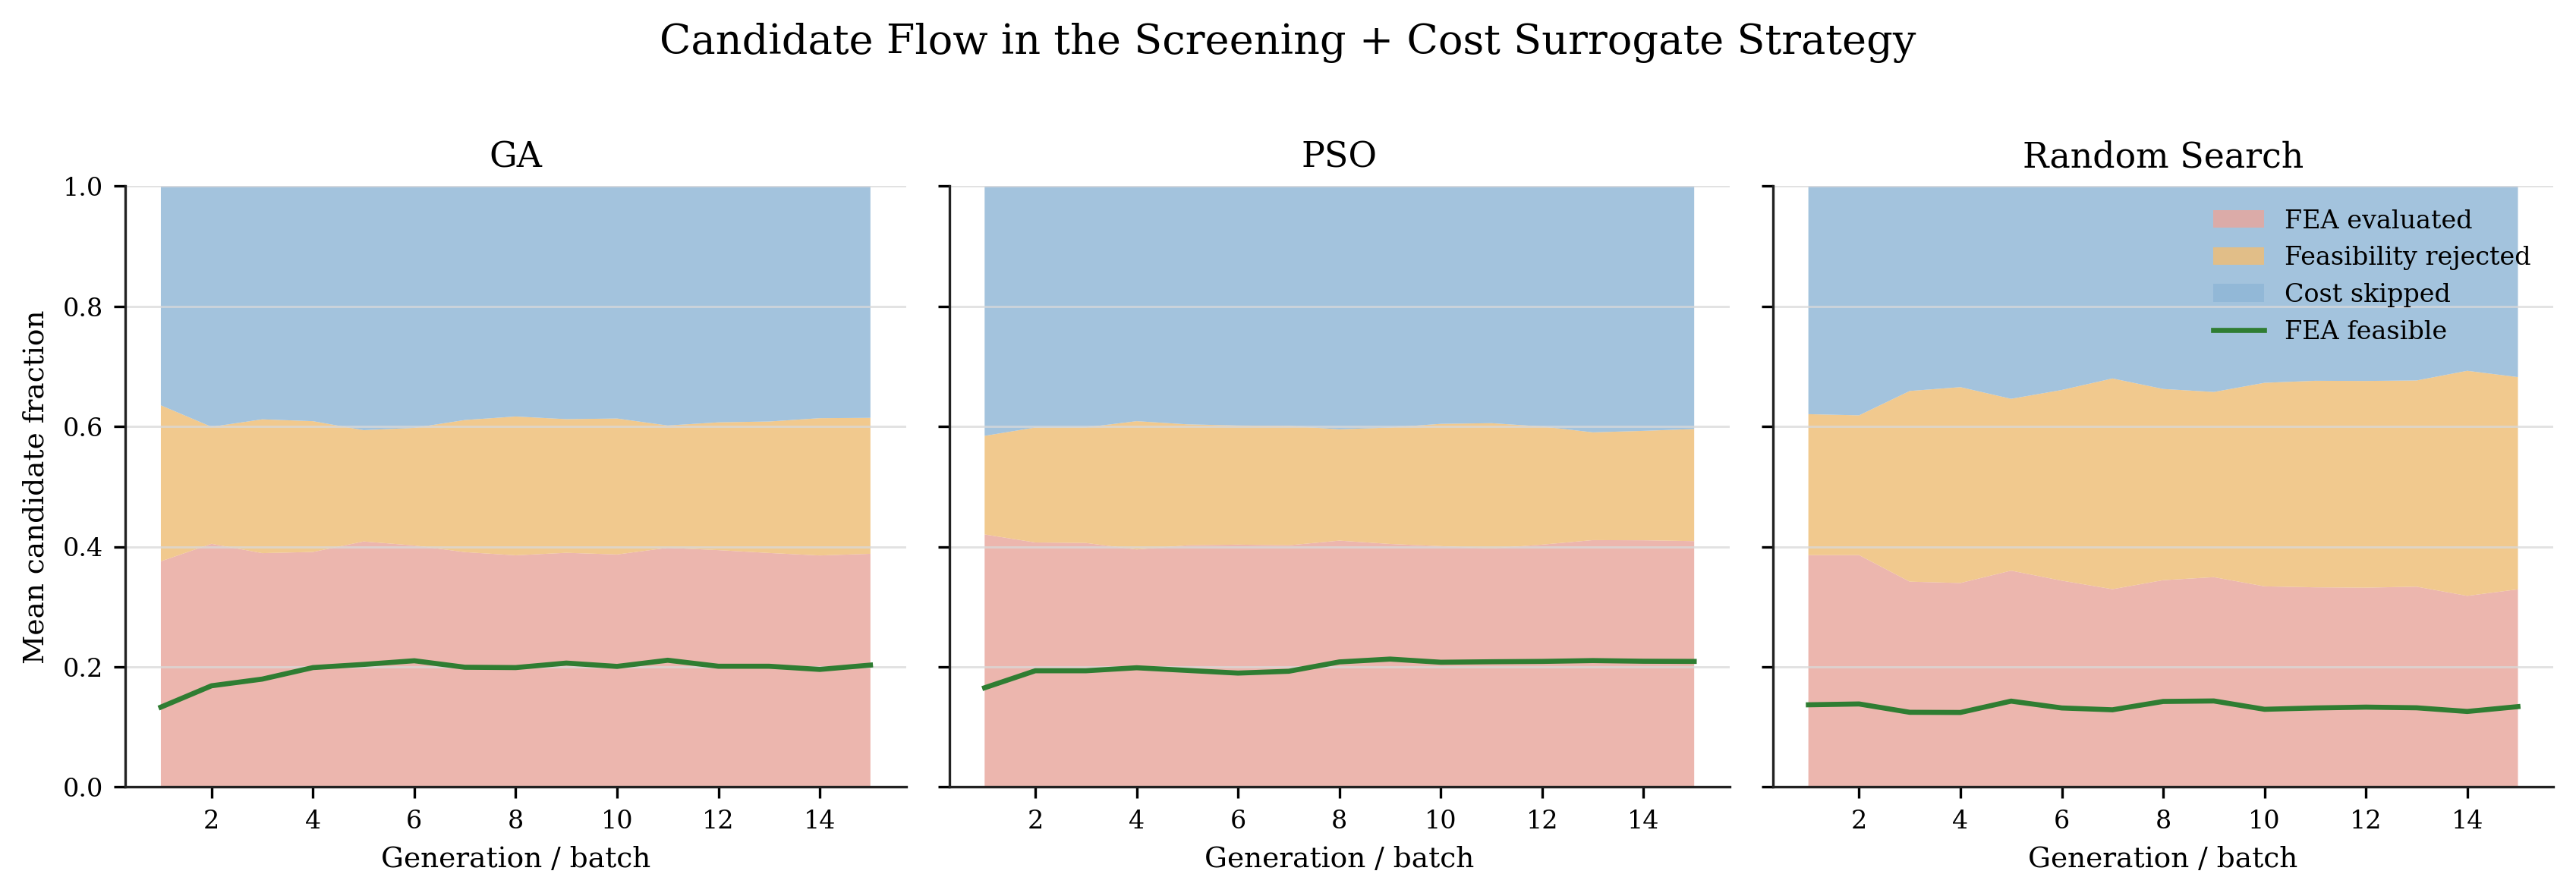
\includegraphics[width=\textwidth,height=0.25\textheight,keepaspectratio]{candidate_flow_analysis.pdf}
\caption{Candidate flow in the calibrated surrogate-informed optimization process.}
\label{fig:candidate_flow_analysis}
\end{figure*}

\begin{figure*}[!t]
\centering
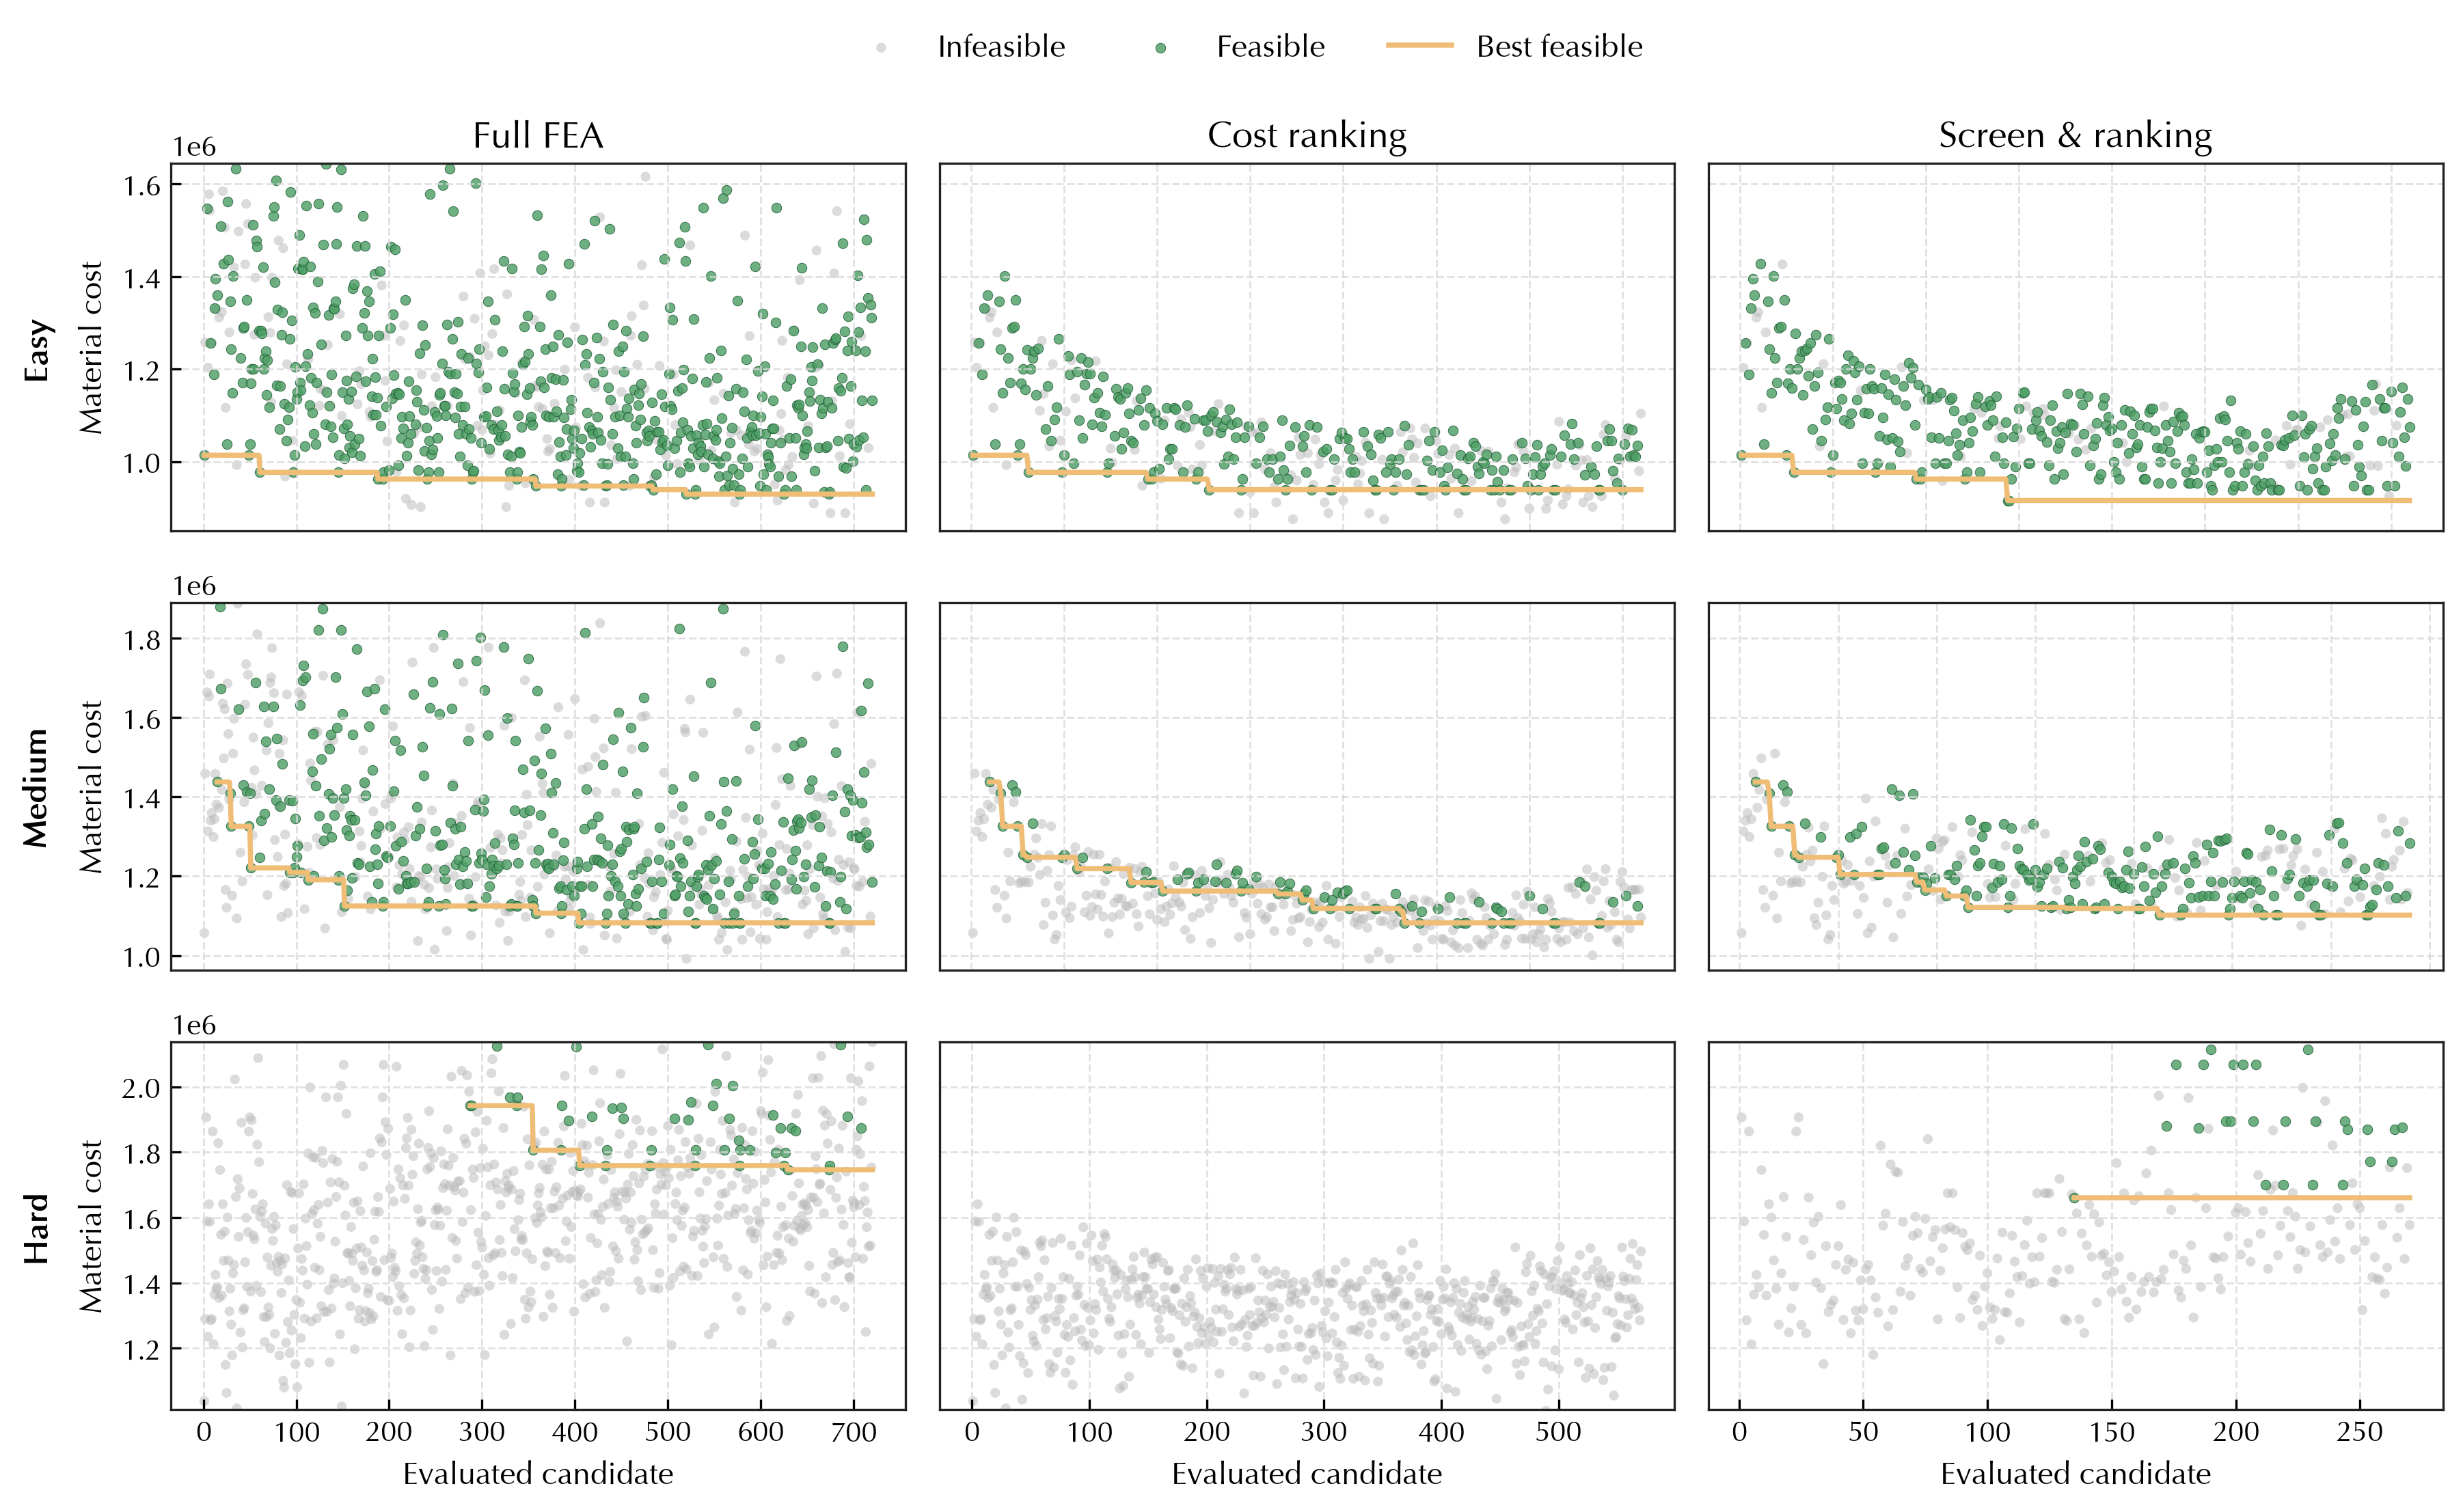
\includegraphics[width=\textwidth]{optimization_case_examples.pdf}
\caption{Representative optimization histories for layouts with different levels of difficulty.}
\label{fig:optimization_case_examples}

\vspace{0.4em}

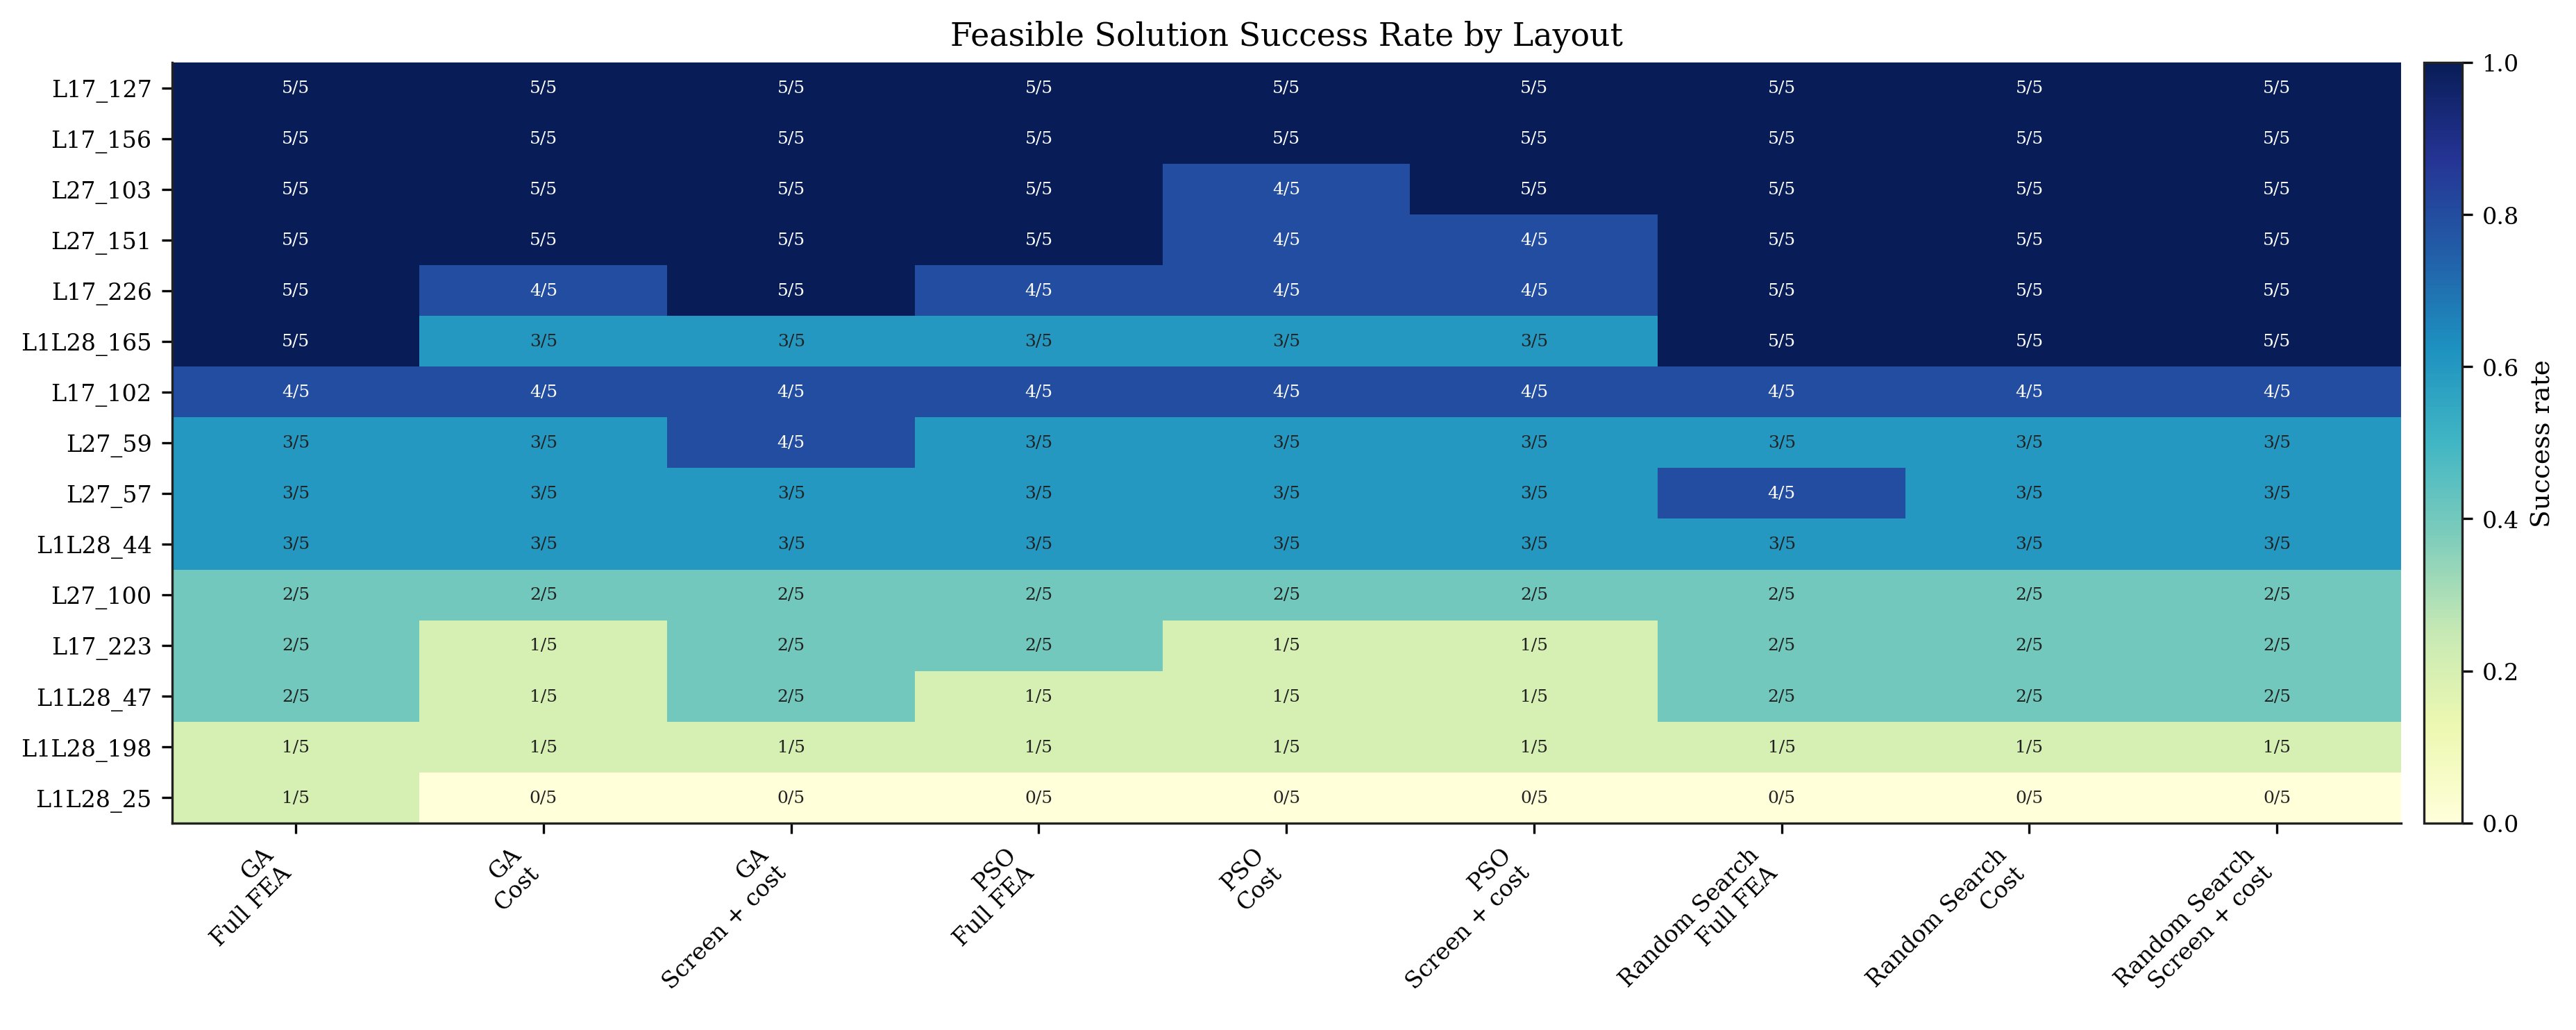
\includegraphics[width=\textwidth]{layout_difficulty_heatmap.pdf}
\caption{Feasible-solution discovery patterns across test layouts and optimization strategies.}
\label{fig:layout_difficulty_heatmap}
\end{figure*}



\subsection{Effectiveness of Online Local Calibration}
\label{subsec:local_calibration_results}
Fig.~\ref{fig:local_calibration_effect} compares the layout-wise prediction errors before and after calibration using 100 local samples. The paired comparisons in Fig.~\ref{fig:local_calibration_effect}(a) and Fig.~\ref{fig:local_calibration_effect}(b) show a consistent shift toward lower error values after calibration, corresponding to lower Brier scores for feasibility prediction and lower MAE for reinforcement estimation. The largest improvements are observed on layouts where the uncalibrated global surrogate has larger errors, indicating that local calibration mainly acts as a bias-correction mechanism rather than replacing the global model.

Table~\ref{tab:local_calibration_results} summarizes representative results using 100 local calibration samples. Three settings are compared to distinguish the effects of global surrogate, direct local learning, and the proposed local calibration strategy. Overall, the calibrated surrogate achieves the best performance for both feasibility prediction and reinforcement estimation.

For the feasibility surrogate, the local-only ablation reduces ECE but does not improve the Brier score, and its feasibility recall is only 0.7265. This result suggests that a model trained only on limited current-layout samples lacks sufficient reliability for conservative screening. In contrast, calibrating the global feasibility probability decreases the Brier score from 0.0749 to 0.0437 and it also decreases the expected calibration error from 0.0895 to 0.0333. The reject rate increases from 0.4708 to 0.5481, while feasibility recall only slightly decreases from 0.9990 to 0.9939. This indicates that calibration improves filtering efficiency while retaining most truly feasible candidates.

For the reinforcement surrogate, the local-only ablation already achieves an MAE of 4.82~t, showing that the mapping from design variables to reinforcement demand can be learned reasonably well within a fixed layout using a small number of samples. Nevertheless, residual calibration of the global prediction further improves both accuracy and bias. The MAE decreases from 11.48~t to 2.04~t, the RMSE decreases from 12.30~t to 2.76~t, and the $R^2$ increases from 0.847 to 0.994. These results confirm that the residual calibration model effectively corrects the systematic error of the global reinforcement surrogate for the current layout.

Fig.~\ref{fig:calibration_sample_efficiency} further examines the sample efficiency of local calibration. The calibration benefit appears with a small number of local samples and then gradually saturates. The feasibility-related results in Fig.~\ref{fig:calibration_sample_efficiency}(a) and Fig.~\ref{fig:calibration_sample_efficiency}(b) show improved probability calibration and screening behavior, while the reinforcement-related results in Fig.~\ref{fig:calibration_sample_efficiency}(c) and Fig.~\ref{fig:calibration_sample_efficiency}(d) show that MAE and bias can be corrected with limited local data. This sample efficiency is important for optimization because the local calibration set is accumulated online from candidates that have already been evaluated by FEA.

Overall, the results confirm that lightweight local calibration can adapt the global surrogate to the current layout without retraining the graph model. Detailed selections of the feasibility probability calibrator and steel residual calibrator under different calibration sample sizes are provided in Appendix Tables~\ref{tab:appendix_feasibility_calibrator} and~\ref{tab:appendix_steel_calibrator}, respectively.

\subsection{Optimization Efficiency and Solution Quality}
\label{subsec:optimization_results}

The calibrated surrogate models are further embedded into optimization procedures to evaluate their practical effect on FEA efficiency and solution quality. 

Table~\ref{tab:optimization_summary_results} summarizes the main quantitative results of the optimization experiments. The cost ratio is computed only for paired cases where both the surrogate-informed strategy and the corresponding full-FEA baseline find feasible solutions. The results show that surrogate-informed evaluation substantially reduces true FEA calls across all three optimizers. The cost-ranking strategy reduces FEA calls by about 50\%--57\%, while adding feasibility screening increases the reduction to about 62\%--66\%. This consistent reduction indicates that the efficiency gain mainly comes from surrogate-based candidate allocation rather than from a specific search algorithm.

The feasible solution discovery rate remains close to that of the full-FEA baseline. With the Screen \& ranking strategy, the success rate decreases only slightly for GA and PSO and remains nearly unchanged for random search. Although surrogate-informed methods may miss feasible designs in some cases, the loss in success rate is small compared with the achieved FEA savings.

Fig.~\ref{fig:optimization_benchmark_results} further compares the distributions of optimization performance. The final material cost results in the second row show that the surrogate-informed strategies do not substantially degrade solution quality. For the Screen \& ranking strategy, the average material cost increase relative to the full-FEA baseline is about 0\%--2\% among paired cases where both strategies find feasible solutions. The first-feasible distributions also show that screening generally reduces the number of FEA calls required to find the first feasible solution, indicating that feasibility prediction helps the optimizer avoid obviously infeasible regions in the early search stage.

In Fig.~\ref{fig:cost_tolerance_analysis}, the horizontal axis represents the allowed cost tolerance relative to the baseline optimum, and the vertical axis represents the proportion of cases that simultaneously satisfy three conditions: a feasible solution is found, the number of FEA calls is reduced, and the final cost is within the specified tolerance. As the tolerance increases from 0\% to about 5\%, the qualified-case ratio increases rapidly and then becomes stable. This trend indicates that, for most cases where full-FEA optimization can find feasible solutions, the surrogate-informed strategy can trade a small cost increase for a substantial reduction in FEA calls.

Taken together, the differences among the three optimizers show that the benefit of surrogate-informed evaluation depends on how effectively each search mechanism uses selectively evaluated candidates. GA benefits most from population diversity and batch-wise comparison, whereas PSO is more sensitive to early screening as the swarm may converge before sufficient calibration samples are accumulated. For random search, the surrogate mainly serves as a pre-evaluation filter because previous evaluations do not guide subsequent sampling. Nevertheless, the consistent reduction in FEA calls across all three optimizers demonstrates that the proposed framework is optimizer-independent in principle. Its fundamental contribution is to increase the information value of each expensive evaluation by directing FEA toward candidates that are more likely to be feasible and economical.

\subsection{Mechanism and Practical Implications}
\label{subsec:mechanism_discussion}

To further clarify how the FEA budget is allocated, Fig.~\ref{fig:candidate_flow_analysis} shows the generation-wise distribution of candidates under the three optimization methods. At each generation or batch, all generated candidates are divided into three mutually exclusive groups: candidates rejected by feasibility screening, candidates that pass the screening but are not selected after cost-based ranking, and candidates submitted to true FEA evaluation. The stacked areas indicate that only approximately 1/3 of the candidates are evaluated by FEA, while the remaining candidates are excluded. The green curve further reports the fraction of candidates that are ultimately confirmed as feasible by FEA. Although the relative proportions differ among GA, PSO, and random search, the overall allocation pattern remains stable throughout optimization, demonstrating that the reduction in FEA calls results from the combined effects of feasibility screening and cost-based ranking.

It is worth noting that some candidates submitted to FEA are still infeasible. This is not a failure of the framework, but a consequence of the conservative screening strategy. The feasibility surrogate is designed to avoid rejecting potentially feasible candidates, so it intentionally retains uncertain or boundary candidates for true verification.

Representative optimization histories are then examined to show how the surrogate modules affect the search trajectory under different layout difficulties. Fig.~\ref{fig:optimization_case_examples} presents three layouts with different feasible candidate ratios, where a higher ratio indicates an easier layout and a lower ratio indicates a more difficult one. In the full FEA baseline, all generated candidates are evaluated, including many high-cost candidates and clearly infeasible candidates. When the reinforcement surrogate is used, evaluations become more concentrated in the low-cost region. However, cost-based ranking alone may still select low-cost but infeasible candidates. After feasibility screening is added, fewer infeasible candidates enter FEA, and the evaluated candidates are more concentrated around promising feasible regions. The best feasible costs remain close to those obtained by full FEA optimization in most cases.

The two surrogate tasks therefore play complementary roles. The reinforcement surrogate reduces evaluations of obviously high-cost candidates and guides the search toward economical designs. The feasibility surrogate reduces evaluations of low-cost but clearly infeasible candidates. Online local calibration further adapts both predictions to the current layout, reducing the influence of global surrogate bias on candidate selection.

As shown in the third row of Fig.~\ref{fig:optimization_case_examples}, the difficult case further reveals why feasibility screening is necessary rather than using cost ranking alone. For this layout, feasible designs are not located in the lowest-cost region; instead, the search needs to move toward larger sections and higher material costs to reach the feasible domain. This trend is evident in the full FEA baseline, where evaluated candidates gradually shift to higher-cost regions and feasible solutions eventually appear. In contrast, the cost-surrogate strategy overemphasizes low-cost candidates, which are mostly infeasible for this layout, and therefore fails to provide useful feedback for moving the search toward feasibility. After feasibility screening is introduced, the screen \& cost ranking strategy filters out low-cost but low-feasibility candidates and retains candidates with higher passing potential. As a result, the search direction becomes closer to the full FEA baseline, enabling feasible solutions to be found with fewer true evaluations.

Finally, layout-level difficulty is analyzed to clarify the applicable scope of the proposed framework. Fig.~\ref{fig:layout_difficulty_heatmap} shows that layout difficulty is a key factor in feasible-solution discovery. Layouts that remain difficult even under full FEA optimization are likely limited by the layout itself or by the section-material design space, rather than by surrogate screening. Therefore, the proposed method is most useful when feasible candidates exist but FEA evaluations are expensive and limited. In such cases, calibrated surrogate can reduce unnecessary evaluations with limited impact on final design quality.
 % discussion

\section{Conclusion}
\label{sec:conclusion}

This study proposed a calibrated surrogate-assisted optimization framework for cross-sectional and material optimization of shear wall structures. A room-graph-based LayoutParamGNN was developed to predict structural feasibility and reinforcement usage, while online local calibration was introduced to correct layout-specific prediction bias using FEA-verified samples accumulated during optimization.

The experimental results lead to the following conclusions:

\begin{enumerate}
\item Layout information is important for surrogate modeling of shear wall structures. The room-graph LayoutParamGNN outperformed models using only design parameters or global layout statistics, achieving a feasibility PR-AUC of 0.8593 and a reinforcement prediction $R^2$ of 0.924 on the test layouts.

\item Online local calibration improves the layout-specific reliability of the global surrogates. With 100 locally verified FEA samples, the feasibility Brier score decreased from 0.0749 to 0.0437, and the reinforcement MAE decreased from 11.48~t to 2.04~t.

\item The calibrated surrogate-assisted strategy substantially reduced FEA calls while maintaining comparable solution quality. Across 15 test layouts and five random seeds, the Screen \& ranking strategy reduced true FEA evaluations by approximately 64.6\% on average, with only a 1.19\% average cost increase in paired feasible cases.

\item The method is most suitable when feasible candidates exist but FEA evaluations are expensive and limited. If the predefined section-material design space contains few or no feasible solutions, surrogate assistance can reduce ineffective evaluations but cannot remove the underlying layout- or design-space limitation.
\end{enumerate}

These findings demonstrate the potential of calibrated surrogate assistance for improving the efficiency of structural design optimization. At the same time, this study is limited to section and material optimization under given shear wall layouts. When the feasible region is extremely small or absent within the predefined design space, surrogate assistance can reduce ineffective evaluations but cannot resolve layout-level infeasibility. In addition, the effectiveness of local calibration depends on the availability and representativeness of FEA-verified samples accumulated during optimization. Future work will extend the framework to joint layout and section optimization, incorporate uncertainty-aware screening to better control false rejection risk, and further validate the method on more complex structural systems and design codes.
 % conclusion
%%%%%%%%%%%%%%%%%%%%%%% main body end %%%%%%%%%%%%%%%%%%%%%%

\section*{Data availability statement}
Data will be made available on request.

\section*{Declaration of Competing Interest}
The authors declare that they have no known competing financial interests or personal relationships that could have appeared to influence the work reported in this paper.

\section*{CRediT authorship contribution statement}
Hao Leng: Conceptualization, Methodology, Software, Formal analysis, Data curation, Writing – original draft \& Visualization. Yuqing Gao: Conceptualization, Methodology, Editing, Review, Supervision. Ying Zhou: Conceptualization, Review, Supervision, Project administration, Funding acquisition. 

\section*{Acknowledgments}
This work was supported by the National Natural Science Foundation of China (No. 52025083, U2139209), the Shanghai Urban Digital Transformation Special Fund (Grant No. 202201033), the Shanghai Rising-Star Program (Grant No. 24YF2749100) and the Open Recruitment for Leadership Positions Project of Tongji Architectural Design (Group) Co., Ltd. (Grant No. 2024J-JB07) . The authors would like to acknowledge Mr. Zhen Zhang, Mr. Yi Wang, Mr. Zhuoju Huang and Mr. Ming Du from Tongji Architectural Design Institute for providing valuable design drawings used to train the model in this study. The authors also thank Dr. Meiyu Du for his helpful suggestions on improvement of the manuscript.


%%%%%%%%%%%%%%%%%%%%%%% appendix %%%%%%%%%%%%%%%%%%%%%%
\clearpage
\onecolumn
\appendix
\setcounter{table}{0}
\renewcommand{\thetable}{A.\arabic{table}}
\renewcommand{\theHtable}{A.\arabic{table}}

\section{Definition of Evaluation Metrics}
\label{app:evaluation_metrics}

This appendix defines the evaluation metrics that are specific to surrogate-assisted candidate screening, probability calibration, ranking-based reinforcement prediction, and optimization efficiency. Standard classification and regression metrics, such as ROC-AUC, PR-AUC, F1 score, MAE, RMSE, $R^2$, and MAPE, follow their conventional definitions and are not repeated here.

\subsection{Screening Metrics for Feasibility Prediction}
\label{app:screening_metrics}

In this study, the feasibility surrogate is used as a conservative screening model. Therefore, its performance is evaluated not only by ordinary classification metrics, but also by whether it can reject low-value candidates while retaining most truly feasible candidates.

Let $y_i \in {0,1}$ denote the true feasibility label of candidate $i$, where $y_i=1$ indicates a feasible candidate. Let $\hat{p}_{f,i}$ denote the predicted or calibrated feasibility probability, and let $\tau$ denote the screening threshold. A candidate is retained for potential FEA evaluation if
\begin{equation}
\hat{p}_{f,i} \geq \tau .
\end{equation}

The feasible recall is defined as
\begin{equation}
R_{\mathrm{fea}}
=
\frac{
\sum_{i=1}^{N}
\mathbb{I}(y_i=1)\mathbb{I}(\hat{p}_{f,i}\geq \tau)
}{
\sum_{i=1}^{N}
\mathbb{I}(y_i=1)
},
\label{eq:app_feasible_recall}
\end{equation}
where $\mathbb{I}(\cdot)$ is the indicator function. This metric measures the proportion of truly feasible candidates retained after surrogate screening. A high feasible recall is required because falsely filtering out feasible candidates may reduce the chance of finding a valid optimal design.

The reject rate is defined as
\begin{equation}
R_{\mathrm{rej}}
=
\frac{
\sum_{i=1}^{N}
\mathbb{I}(\hat{p}_{f,i}<\tau)
}{N}.
\label{eq:app_reject_rate}
\end{equation}
It measures the proportion of candidates rejected before true FEA evaluation. A higher reject rate indicates greater potential for reducing FEA calls, but it is meaningful only when feasible recall remains sufficiently high.

The false reject count is defined as
\begin{equation}
N_{\mathrm{fr}}
=
\sum_{i=1}^{N}
\mathbb{I}(y_i=1)\mathbb{I}(\hat{p}_{f,i}<\tau).
\label{eq:app_false_reject}
\end{equation}
It directly counts the number of truly feasible candidates incorrectly rejected by the screening rule. This metric is reported because even a small false reject rate may be important when the number of feasible candidates is limited.

\subsection{Probability Calibration Metrics}
\label{app:calibration_metrics}

The feasibility surrogate outputs a probability rather than a binary decision. In surrogate-assisted optimization, probability reliability is important because the screening threshold is selected based on predicted feasibility probabilities.

The Brier score is used to measure the mean squared error between predicted probabilities and true binary labels:
\begin{equation}
\mathrm{Brier}
=
\frac{1}{N}
\sum_{i=1}^{N}
(\hat{p}_{f,i}-y_i)^2.
\label{eq:app_brier}
\end{equation}
A lower Brier score indicates better probabilistic prediction.

Expected calibration error (ECE) measures the discrepancy between predicted probability and empirical feasibility frequency. The predictions are divided into $M$ probability bins. Let $B_m$ denote the set of samples in bin $m$. The average confidence and empirical feasible rate in bin $m$ are defined as
\begin{equation}
\mathrm{conf}(B_m)
=
\frac{1}{|B_m|}
\sum_{i\in B_m}
\hat{p}_{f,i},
\label{eq:app_confidence}
\end{equation}
\begin{equation}
\mathrm{freq}(B_m)
=
\frac{1}{|B_m|}
\sum_{i\in B_m}
y_i.
\label{eq:app_frequency}
\end{equation}
The ECE is then calculated as
\begin{equation}
\mathrm{ECE}
=
\sum_{m=1}^{M}
\frac{|B_m|}{N}
\left|
\mathrm{freq}(B_m)
-
\mathrm{conf}(B_m)
\right|.
\label{eq:app_ece}
\end{equation}
A smaller ECE indicates that the predicted feasibility probabilities are more consistent with the observed feasible frequencies.

\subsection{Ranking Metrics for Reinforcement Prediction}
\label{app:ranking_metrics}

The reinforcement surrogate is mainly used to rank candidates by material economy before true FEA evaluation. Therefore, ranking-oriented metrics are reported in addition to regression errors.

Pairwise ranking accuracy evaluates whether the surrogate correctly predicts the relative order of reinforcement usage between candidate pairs. Given two candidates $i$ and $j$, the ordering is correctly predicted if
\begin{equation}
(m_{s,i}-m_{s,j})(\hat{m}_{s,i}-\hat{m}_{s,j}) > 0 .
\end{equation}
The pairwise ranking accuracy is defined as
\begin{equation}
A_{\mathrm{rank}}
=
\frac{
\sum_{i<j}
\mathbb{I}
\left[
(m_{s,i}-m_{s,j})(\hat{m}_{s,i}-\hat{m}_{s,j}) > 0
\right]
}{
\binom{N}{2}
}.
\label{eq:app_pairwise_ranking}
\end{equation}
A higher value indicates that the surrogate better preserves the relative material economy of candidates.

Spearman's rank correlation coefficient is also used to measure the monotonic agreement between true and predicted reinforcement usage:
\begin{equation}
\rho_s
=
1
-
\frac{
6\sum_{i=1}^{N} d_i^2
}{
N(N^2-1)
},
\label{eq:app_spearman}
\end{equation}
where $d_i$ is the difference between the true rank and predicted rank of candidate $i$. A value closer to 1 indicates better rank consistency.

Top-$k$ recall evaluates whether the surrogate can identify the truly low-reinforcement candidates. Let $\mathcal{T}_k$ denote the set of candidates with the lowest true reinforcement usage, and let $\hat{\mathcal{T}}_k$ denote the set of candidates with the lowest predicted reinforcement usage. The top-$k$ recall is defined as
\begin{equation}
R_{\mathrm{top}\text{-}k}
=
\frac{
|\mathcal{T}_k \cap \hat{\mathcal{T}}_k|
}{
|\mathcal{T}_k|
}.
\label{eq:app_topk_recall}
\end{equation}
This metric is particularly relevant for optimization because only a small subset of promising candidates is selected for true FEA evaluation.

The prediction bias of reinforcement usage is defined as
\begin{equation}
\mathrm{Bias}
=
\frac{1}{N}
\sum_{i=1}^{N}
(\hat{m}_{s,i}-m_{s,i}).
\label{eq:app_bias}
\end{equation}
A positive value indicates overestimation, while a negative value indicates underestimation. Bias is reported because systematic overestimation or underestimation may affect candidate ranking and FEA budget allocation.

\subsection{Optimization Efficiency and Solution Quality Metrics}
\label{app:optimization_metrics}

In the optimization experiments, the primary computational metric is the number of true FEA calls:
\begin{equation}
N_{\mathrm{FEA}}
=
\sum_{t}
|\mathcal{S}_t|,
\label{eq:app_fea_calls}
\end{equation}
where $\mathcal{S}_t$ is the set of candidates submitted to the true evaluator at iteration $t$.

The FEA reduction ratio is calculated relative to full FEA optimization:
\begin{equation}
R_{\mathrm{FEA}}
=
1
-
\frac{
N_{\mathrm{FEA}}^{\mathrm{sur}}
}{
N_{\mathrm{FEA}}^{\mathrm{full}}
},
\label{eq:app_fea_reduction}
\end{equation}
where $N_{\mathrm{FEA}}^{\mathrm{sur}}$ and $N_{\mathrm{FEA}}^{\mathrm{full}}$ are the numbers of true FEA calls used by the surrogate-assisted strategy and the full FEA baseline, respectively.

The feasible-solution discovery rate is defined as the proportion of optimization runs that successfully find at least one feasible design:
\begin{equation}
R_{\mathrm{succ}}
=
\frac{
N_{\mathrm{runs}}^{\mathrm{feasible}}
}{
N_{\mathrm{runs}}
}.
\label{eq:app_success_rate}
\end{equation}
This metric reflects whether surrogate screening reduces the chance of discovering feasible solutions.

For runs that find feasible solutions, the final material cost of the best FEA-verified feasible design is reported. To compare surrogate-assisted optimization with full FEA optimization under the same layout and random seed, the normalized objective ratio is calculated as
\begin{equation}
R_{\mathrm{obj}}
=
\frac{
C_{\mathrm{best}}^{\mathrm{sur}}
}{
C_{\mathrm{best}}^{\mathrm{full}}
},
\label{eq:app_objective_ratio}
\end{equation}
where $C_{\mathrm{best}}^{\mathrm{sur}}$ and $C_{\mathrm{best}}^{\mathrm{full}}$ are the best verified feasible costs obtained by the surrogate-assisted method and the full FEA baseline, respectively. A value close to 1 indicates that the surrogate-assisted method achieves comparable solution quality.

The number of FEA calls required to find the first feasible solution is also reported:
\begin{equation}
N_{\mathrm{first}}
=
\min
\left\{
n
\mid
\exists i \leq n,\ y_{f,i}=1
\right\}.
\label{eq:app_first_feasible}
\end{equation}
This metric indicates how quickly an optimization strategy reaches the feasible region under a limited FEA budget.


\section{Additional Calibration Results}
\label{app:calibration_results}
\setcounter{table}{0}
\renewcommand{\thetable}{B.\arabic{table}}
\renewcommand{\theHtable}{B.\arabic{table}}

Tables~\ref{tab:appendix_feasibility_calibrator} and~\ref{tab:appendix_steel_calibrator} report the calibration-model selection results for feasibility probability calibration and steel-usage residual calibration under different local sample sizes. For each sample size, several lightweight calibrators are trained and the model with the best Brier score is reported together with other evaluation metrics. The results show that the most suitable calibrator varies with the amount of available local calibration data.

\begin{table}[H]
\centering
\caption{Best feasibility probability calibrator under different local sample sizes.}
\label{tab:appendix_feasibility_calibrator}
\small
\setlength{\tabcolsep}{6pt}
\begin{tabularx}{\textwidth}{@{}>{\centering\arraybackslash}p{0.12\textwidth}
>{\raggedright\arraybackslash}X
>{\centering\arraybackslash}p{0.10\textwidth}
>{\centering\arraybackslash}p{0.09\textwidth}
>{\centering\arraybackslash}p{0.13\textwidth}
>{\centering\arraybackslash}p{0.13\textwidth}@{}}
\toprule
Calib. samples & Best feasibility calibrator & Brier & ECE & Screen reject & Screen recall \\
\midrule
25 & Platt scaling & 0.0505 & 0.0455 & 47.4\% & 0.9476 \\
50 & Residual random forest & 0.0464 & 0.0406 & 51.6\% & 0.9485 \\
100 & Residual random forest & 0.0420 & 0.0325 & 52.3\% & 0.9487 \\
200 & Residual random forest & 0.0381 & 0.0261 & 59.1\% & 0.9481 \\
500 & Residual random forest & 0.0344 & 0.0201 & 63.9\% & 0.9441 \\
\bottomrule
\end{tabularx}
\end{table}

\begin{table}[H]
\centering
\caption{Best steel residual calibrator under different local sample sizes.}
\label{tab:appendix_steel_calibrator}
\small
\setlength{\tabcolsep}{6pt}
\begin{tabularx}{\textwidth}{@{}>{\centering\arraybackslash}p{0.12\textwidth}
>{\raggedright\arraybackslash}X
>{\centering\arraybackslash}p{0.12\textwidth}
>{\centering\arraybackslash}p{0.12\textwidth}
>{\centering\arraybackslash}p{0.08\textwidth}
>{\centering\arraybackslash}p{0.11\textwidth}@{}}
\toprule
Calib. samples & Best steel residual model & MAE (kg) & RMSE (kg) & $R^2$ & Pair acc. \\
\midrule
25 & Ridge & 2395.9 & 3162.8 & 0.9924 & 0.9769 \\
50 & Gaussian process & 2229.1 & 3003.6 & 0.9932 & 0.9785 \\
100 & Gaussian process & 2044.7 & 2756.0 & 0.9943 & 0.9797 \\
200 & LightGBM & 1741.3 & 2386.0 & 0.9957 & 0.9821 \\
500 & LightGBM & 1444.8 & 1992.6 & 0.9970 & 0.9851 \\
\bottomrule
\end{tabularx}
\end{table}

\clearpage

%%%%%%%%%%%%%%%%%%%%%%% bibliography %%%%%%%%%%%%%%%%%%%%%%
\twocolumn
%% If you have bibdatabase file and want bibtex to generate the
%% bibitems, please use
%%
\bibliographystyle{elsarticle-num} 
\bibliography{cas-refs}

%% else use the following coding to input the bibitems directly in the
%% TeX file.

% \begin{thebibliography}{00}

% %% \bibitem{label}
% %% Text of bibliographic item

% \bibitem{}

% \end{thebibliography}
\end{document}
\endinput
%%
%% End of file `elsarticle-template-num.tex'.
